% CVPR 2025 Paper Template; see https://github.com/cvpr-org/author-kit

\documentclass[10pt,twocolumn,letterpaper,table]{article}

%%%%%%%%% PAPER TYPE  - PLEASE UPDATE FOR FINAL VERSION
% \usepackage{cvpr}              % To produce the CAMERA-READY version
% \usepackage[review]{cvpr}      % To produce the REVIEW version
\usepackage[pagenumbers]{cvpr} % To force page numbers, e.g. for an arXiv version
\usepackage{multirow}
\usepackage{xcolor}
% \usepackage{array}
% \usepackage[accsupp]{axessibility}

% Import additional packages in the preamble file, before hyperref
%
% --- inline annotations
%
\newcommand{\red}[1]{{\color{red}#1}}
\newcommand{\todo}[1]{{\color{red}#1}}
\newcommand{\TODO}[1]{\textbf{\color{red}[TODO: #1]}}
% --- disable by uncommenting  
% \renewcommand{\TODO}[1]{}
% \renewcommand{\todo}[1]{#1}

\usepackage{xcolor}
\usepackage{graphicx}
\usepackage{booktabs}
\usepackage{amsmath} 
\usepackage{amsfonts}
\usepackage{amssymb}
\usepackage{multirow} 
\usepackage{makecell}
\newcommand{\shline}{\Xhline{1.1pt}} % Adjust thickness as desired

% It is strongly recommended to use hyperref, especially for the review version.
% hyperref with option pagebackref eases the reviewers' job.
% Please disable hyperref *only* if you encounter grave issues, 
% e.g. with the file validation for the camera-ready version.
%
% If you comment hyperref and then uncomment it, you should delete *.aux before re-running LaTeX.
% (Or just hit 'q' on the first LaTeX run, let it finish, and you should be clear).
\definecolor{cvprblue}{rgb}{0.21,0.49,0.74}
\usepackage[pagebackref,breaklinks,colorlinks,allcolors=cvprblue]{hyperref}

%%%%%%%%% PAPER ID  - PLEASE UPDATE
% \def\paperID{7929} % *** Enter the Paper ID here
% \def\confName{CVPR}
% \def\confYear{2025}

\renewcommand{\thefootnote}{}
\newcommand{\name}{STAR}
% \newcommand{\name}{$\mathtt{STAR}$}
%%%%%%%%% TITLE - PLEASE UPDATE
\title{STAR: Spatial-Temporal Augmentation with Text-to-Video Models\\ for Real-World Video Super-Resolution}

%%%%%%%%% AUTHORS - PLEASE UPDATE
\author{
  Rui Xie$^{1*}$, \hspace{0.2cm}
  Yinhong Liu$^{1*}$, \hspace{0.2cm}
  Penghao Zhou$^2$, \hspace{0.2cm}
  Chen Zhao$^1$, \hspace{0.2cm}
  Jun Zhou$^3$ \\
  Kai Zhang$^1$, \hspace{0.2cm}
  Zhenyu Zhang$^1$, \hspace{0.2cm}
  Jian Yang$^{1}$, \hspace{0.2cm}
  Zhenheng Yang$^2$, \hspace{0.2cm}
  Ying Tai$^{1\dagger}$ \\
  $^1$Nanjing University, \hspace{0.2cm}
  $^2$ByteDance, \hspace{0.2cm}
  $^3$Southwest University \\
  {\small \url{https://nju-pcalab.github.io/projects/STAR}}
}


\begin{document}
% \maketitle

\twocolumn[{
\renewcommand\twocolumn[1][]{#1}
\maketitle
\begin{center}
    \captionsetup{type=figure}
    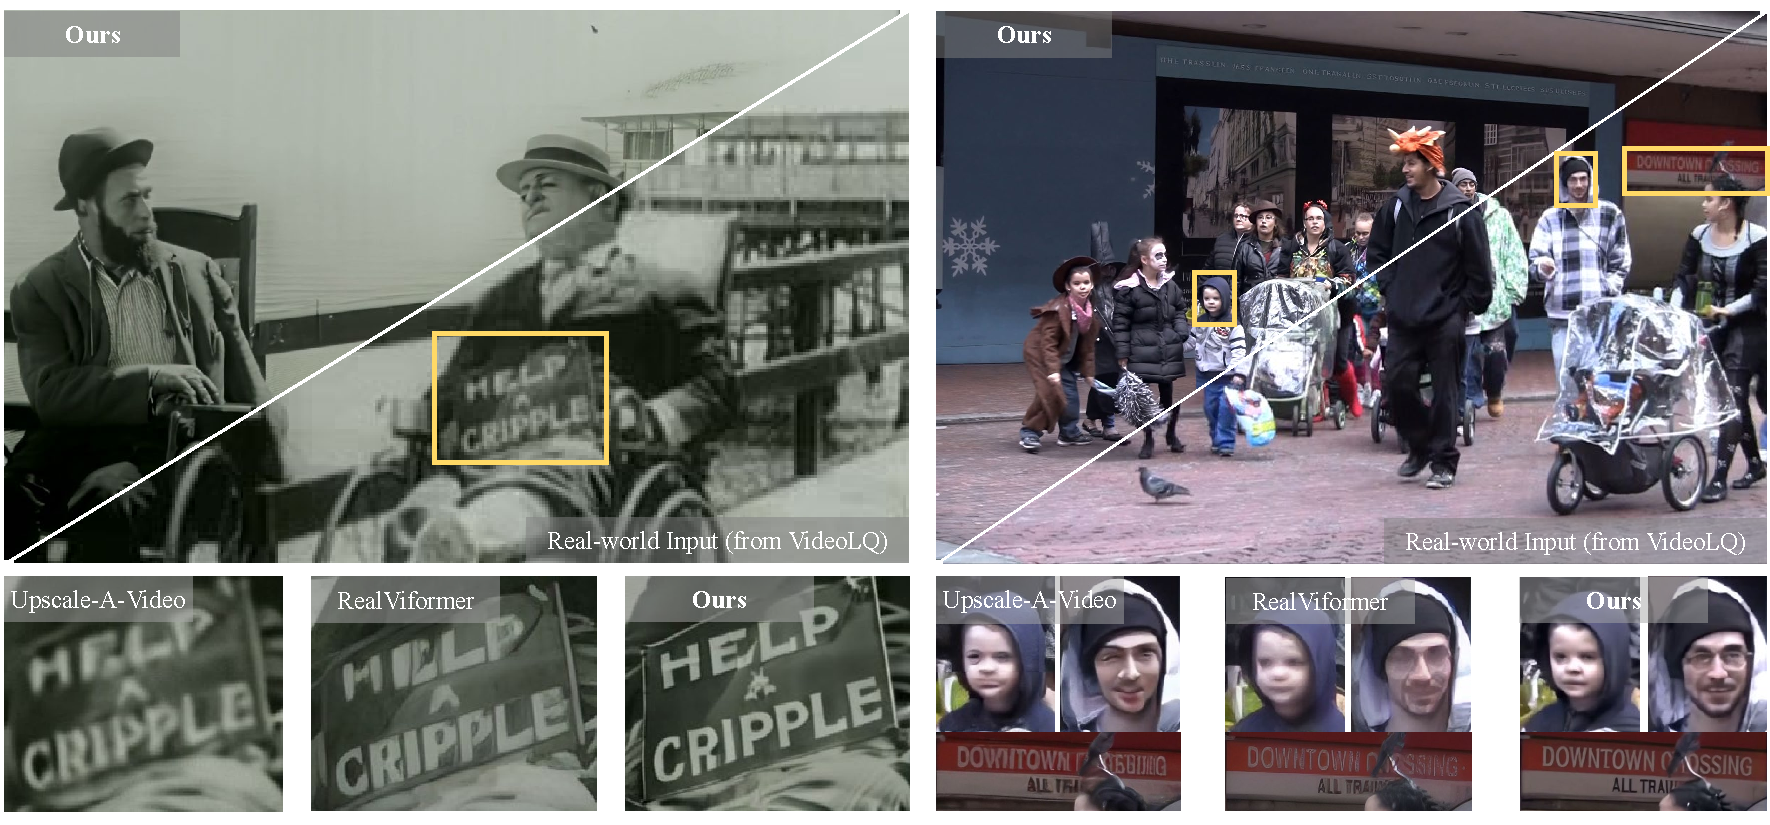
\includegraphics[width=\textwidth]{figure/figure1.pdf} \vspace{-6mm}
    \captionof{figure}{Visualization comparisons on both real-world and synthetic low-resolution videos. 
    Compared to the state-of-the-art VSR models~\cite{zhang2024realviformer,zhou2024upscale}, our results demonstrate more natural facial details and better structure of the text. 
    \textbf{(Zoom-in for best view)}}
    \label{teaser}
\end{center}
}]

\begin{abstract}
Segment Anything Model 2 (SAM 2) has emerged as a powerful tool for video object segmentation and tracking anything. Key components of SAM 2 that drive the impressive video object segmentation performance include a large multistage image encoder for frame feature extraction and a memory mechanism that stores memory contexts from past frames to help current frame segmentation. The high computation complexity of multistage image encoder and memory module has limited its applications in real-world tasks, e.g., video object segmentation on mobile devices. To address this limitation, we propose EfficientTAMs, lightweight track anything models that produce high-quality results with low latency and model size. Our idea is based on revisiting the plain, nonhierarchical Vision Transformer (ViT) as an image encoder for video object segmentation, and introducing an efficient memory module, which reduces the complexity for both frame feature extraction and memory computation for current frame segmentation. We take vanilla lightweight ViTs and efficient memory module to build EfficientTAMs, and train the models on SA-1B and SA-V datasets for video object segmentation and track anything tasks. We evaluate on multiple video segmentation benchmarks including semi-supervised VOS and promptable video segmentation, and find that our proposed EfficientTAM with vanilla ViT perform comparably to SAM 2 model (HieraB+SAM 2) with $\sim$2x speedup on A100 and $\sim$2.4x  parameter reduction. On segment anything image tasks, our EfficientTAMs also perform favorably over original SAM with $\sim$20x  speedup on A100 and $\sim$20x  parameter reduction. On mobile devices such as iPhone 15 Pro Max, our EfficientTAMs can run at $\sim$10 FPS for performing video object segmentation with reasonable quality, highlighting the capability of small models for on-device video object segmentation applications. 
\end{abstract}
\section{Introduction}
Deep learning techniques have made rapid progress in conditional image generation. For example, networks have been used to inpaint missing image regions~\citep{pathakCVPR16context,yang2016high,isola2016image}, 
add color to grayscale images~\citep{iizuka2016let,larsson2016learning,zhang2016colorful,isola2016image}, and generate photorealistic images from sketches~\cite{sangkloy2017scribbler,isola2016image}.
However, most techniques in this space have focused on generating a \textit{single} result.
In this work, we model a \textit{distribution} of potential results, as many of these problems may be multimodal in nature. For example,
as seen in Figure~\ref{fig:teaser}, an image captured at night may look very different in the day, depending on cloud patterns and lighting conditions.
We pursue two main goals: producing results which are (1) perceptually realistic and (2) diverse, all while remaining faithful to the input.

Mapping from a high-dimensional input to a high-dimensional output distribution is challenging. A common approach to representing multimodality is learning a low-dimensional latent code, which should represent aspects of the possible outputs not contained in the input image. At inference time, a deterministic generator uses the input image, along with stochastically sampled latent codes, to produce randomly sampled outputs. A common problem in existing methods is~\textit{mode collapse}~\citep{goodfellow2016nips}, where only a small number of real samples get represented in the output.
We systematically study a family of solutions to this problem.

We start with the \pp framework~\citep{isola2016image}, which has previously been shown to produce high-quality results for various image-to-image translation tasks. The method trains a generator network, conditioned on the input image, with two losses: (1) a regression loss to produce similar output to the known paired ground truth image and (2) a learned discriminator loss to encourage realism. The authors note that trivially appending a randomly drawn latent code did not produce diverse results. Instead, we propose encouraging a bijection between the output and latent space. 
We not only perform the direct task of mapping the latent code (along with the input) to the output but also jointly learn an encoder from the output back to the latent space. 
This discourages two different latent codes from generating the same output (non-injective mapping).
During training, the learned encoder attempts to pass enough information to the generator to resolve any ambiguities regarding the output mode.
For example, when generating a day image from a night image, the latent vector may encode information about the sky color, lighting effects on the ground, and cloud patterns.  Composing the encoder and generator sequentially should result in the same image being recovered. The opposite should produce the same latent code.

\begin{figure}
\centering
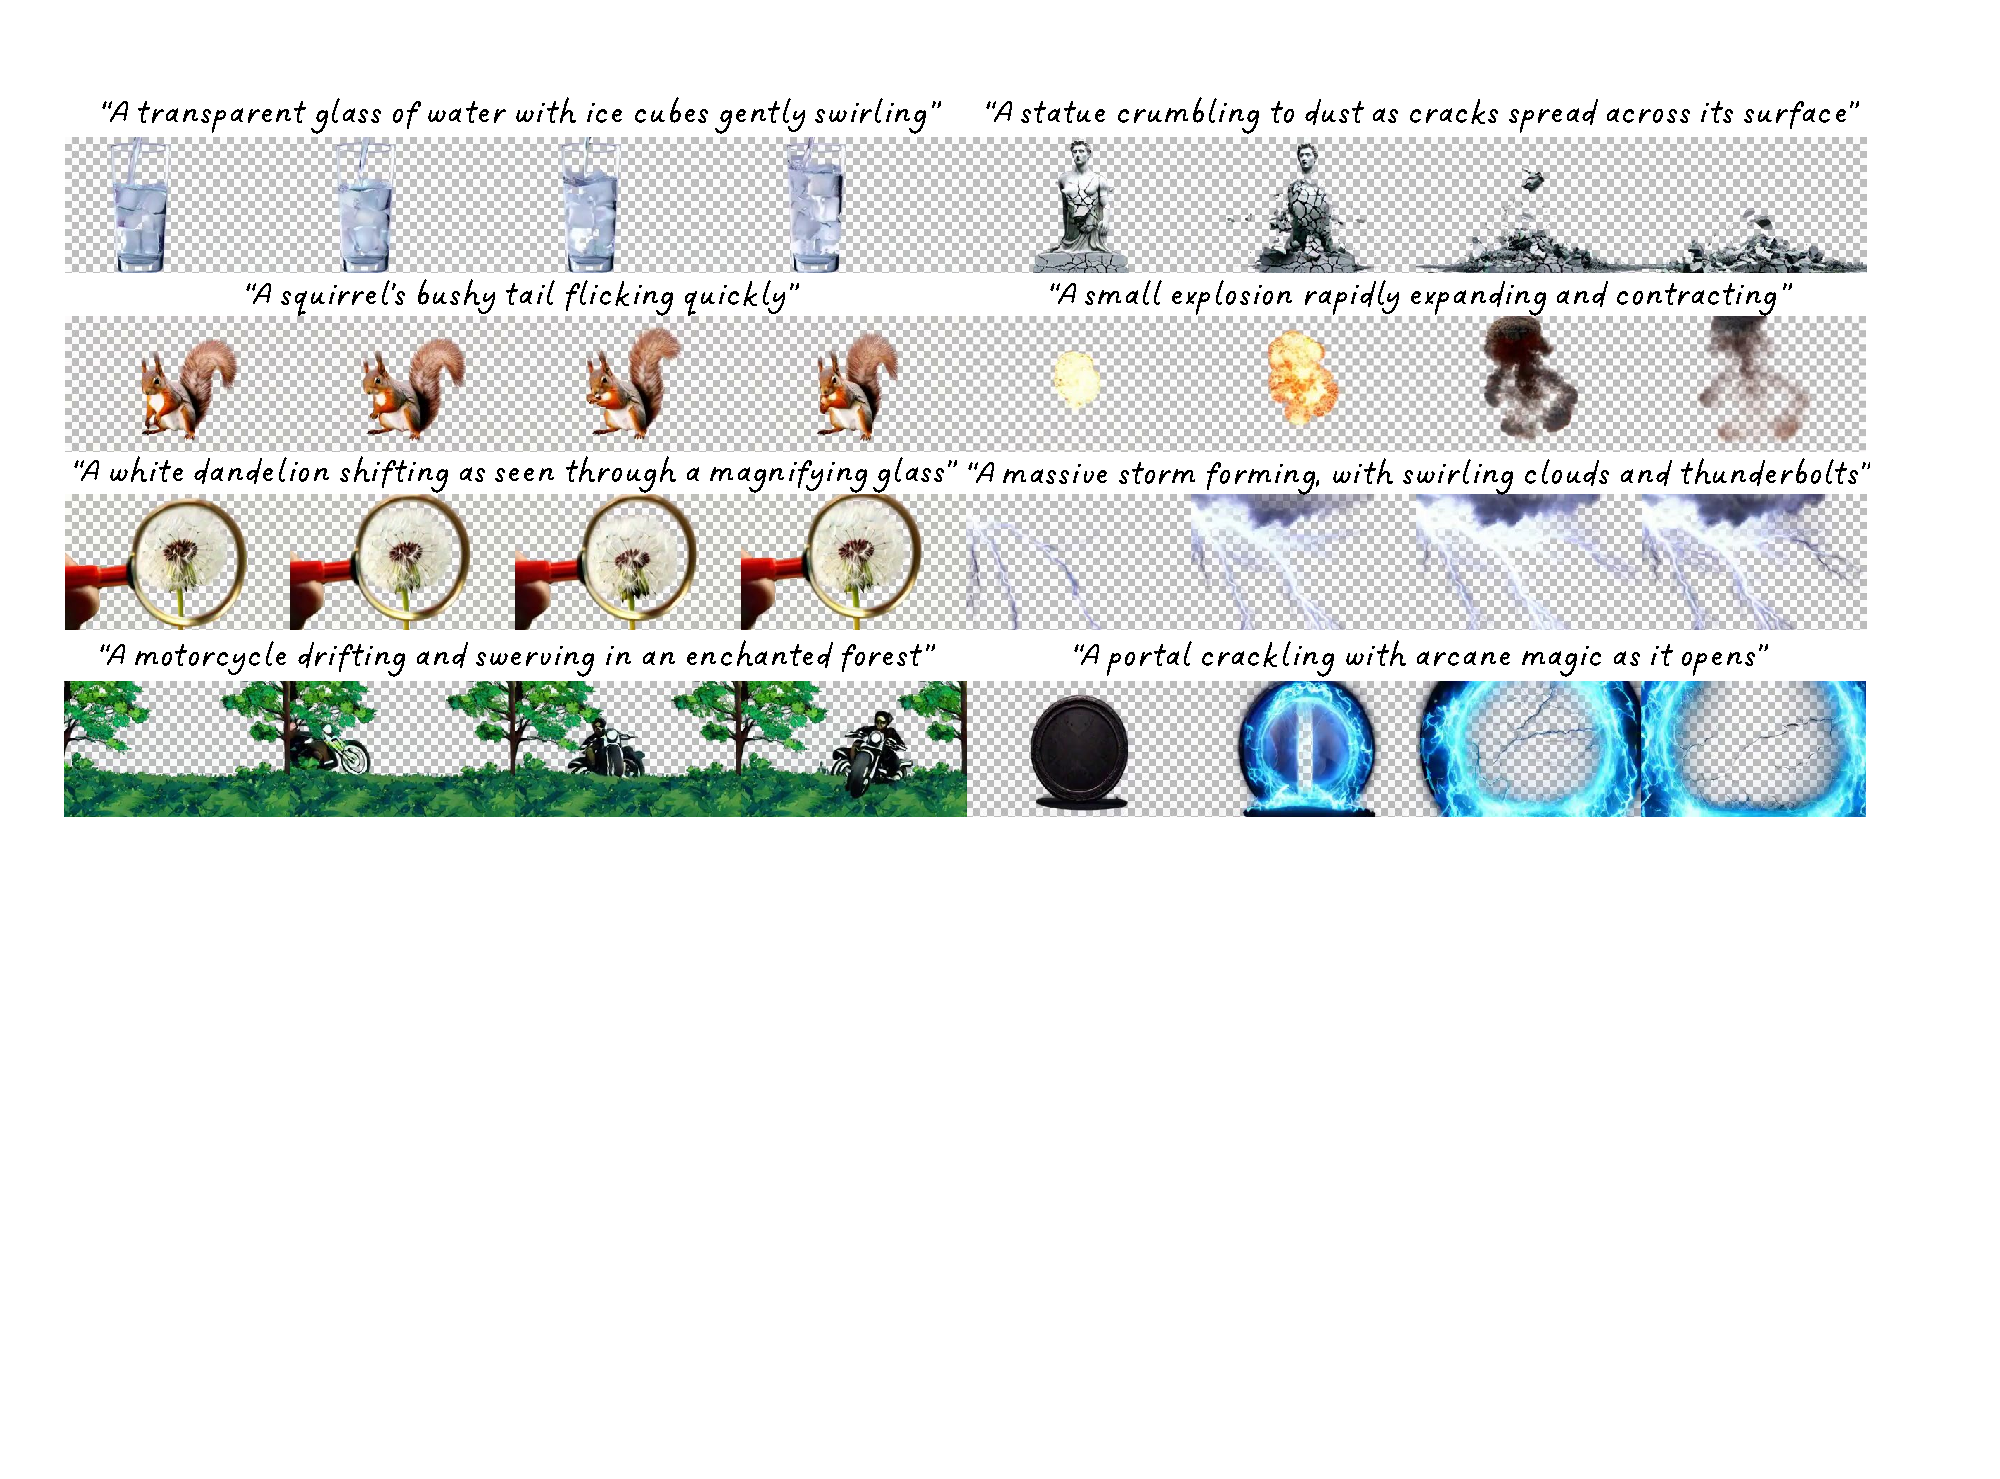
\includegraphics[width=1.\linewidth]{imgs/teaser.pdf}
\vspace{-4mm}
\caption{\small Multimodal image-to-image translation using our proposed method: given an input image from one domain (night image of a scene), we aim to model a \textit{distribution} of potential outputs in the target domain (corresponding day images), producing both realistic and diverse results.}
\vspace{-4mm}
\label{fig:teaser}
\end{figure}


In this work, we instantiate this idea by exploring several objective functions, inspired by literature in unconditional generative modeling:
  \begin{itemize}[leftmargin=0.1in]
  
    \item \textbf{\cvaegan (Conditional Variational Autoencoder GAN)}:
    One approach is first encoding the ground truth image into the latent space, giving the generator a noisy ``peek" into the desired output. Using this, along with the input image, the generator should be able to reconstruct the specific output image. To ensure that random sampling can be used during inference time, the latent distribution is regularized using KL-divergence to be close to a standard normal distribution. This approach has been popularized in the unconditional setting by VAEs~\citep{kingma2013auto} and VAE-GANs~\citep{larsen2016vaegan}.
    
    \item \textbf{\cinfogan (Conditional Latent Regressor GAN)}: Another approach is to first provide a randomly drawn latent vector to the generator. In this case, the produced output may not necessarily look like the ground truth image, but it should look realistic. An encoder then attempts to recover the latent vector from the output image. This method could be seen as a conditional formulation of the ``latent regressor" model~\citep{donahue2016adversarial,dumoulin2016adversarially} and also related to InfoGAN~\citep{xi2016infogan}.
    
    \item \textbf{\bicycle}: Finally, we combine both these approaches to enforce the connection between latent encoding and output in both directions {\em jointly} and achieve improved performance. We show that our method can produce both diverse and visually appealing results across a wide range of image-to-image translation problems, significantly more diverse than other baselines, including naively adding noise in the \pp framework. In addition to the loss function, we study the performance with respect to several encoder networks, as well as different ways of injecting the latent code into the generator network. 
\end{itemize}

We perform a systematic evaluation of these variants by using humans to judge photorealism and a perceptual distance metric~\cite{zhang2018unreasonable} to assess output diversity. Code and data are available at \url{https://github.com/junyanz/BicycleGAN}.
\section{Related Work}
\label{sec:related work}

\begin{figure*}[t]
    \centering
    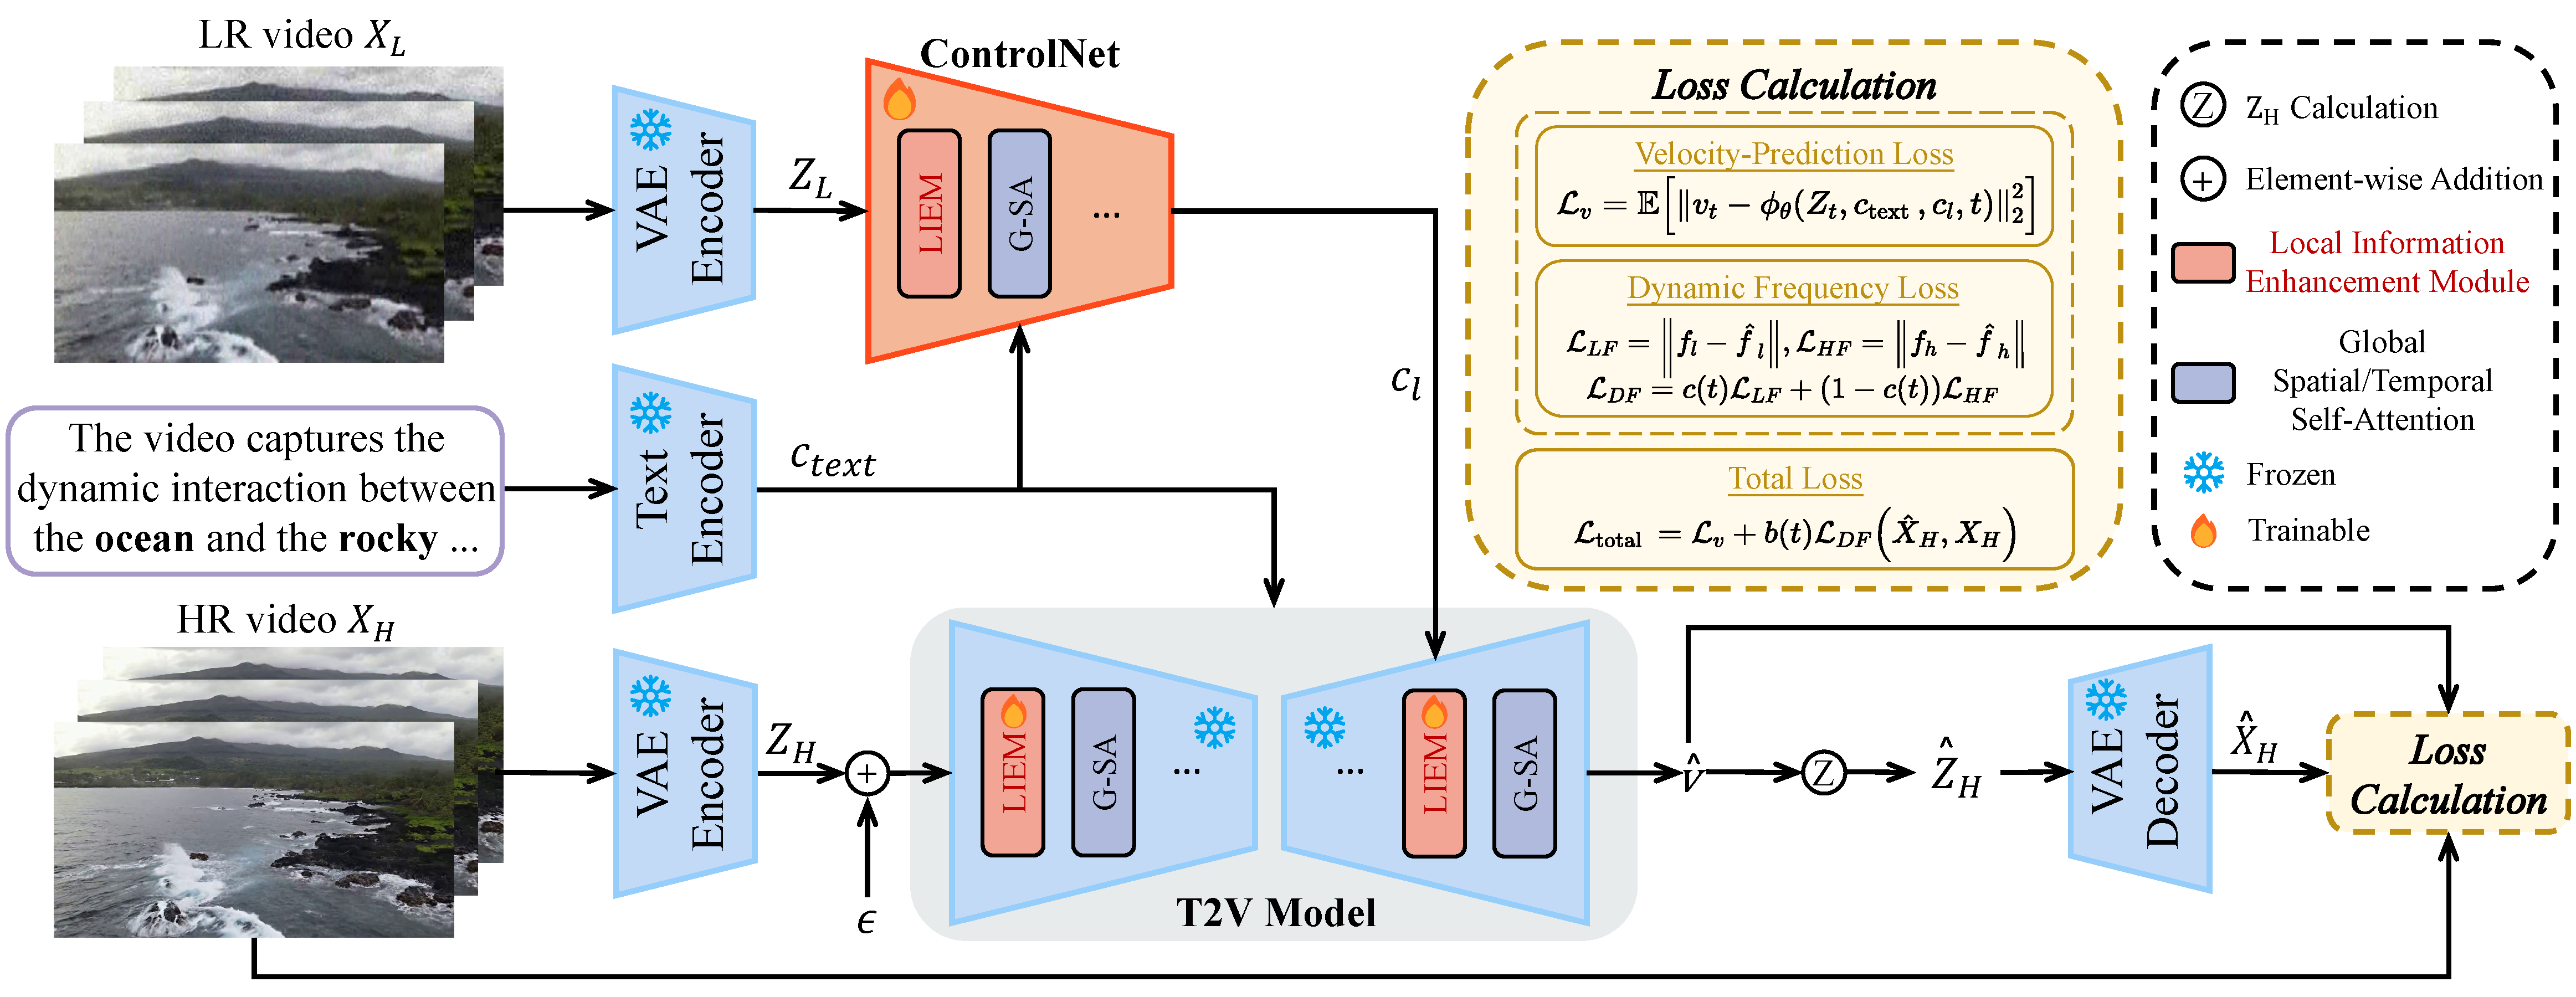
\includegraphics[width=1\linewidth]{figure/overview.pdf}\vspace{-2mm}
    \caption{Overview of the proposed~\name.}
    \label{fig:overview}
\end{figure*}

% \textbf{Video Super-Resolution.}
\paragraph{Video Super-Resolution.} 
Traditional VSR methods can be roughly divided into two categories: recurrent-based \cite{haris2019recurrent, huang2017video, liang2022recurrent, sajjadi2018frame, shi2022rethinking} and sliding-window-based \cite{caballero2017real,liang2024vrt,li2020mucan,xu2021temporal,yi2019progressive} methods. 
Recurrent-based methods process LR video frame by frame using recurrent neural networks \cite{mikolov2010recurrent}. In contrast, sliding-window-based methods divide a video sequence into segments, using each as input to super-resolve the video. 
However, both approaches suffer from degradation mismatch, leading to significant performance drops in real-world applications.
Recently, there has been a growing focus on real-world VSR, targeting complex, unknown degradations. RealBasicVSR \cite{chan2022investigating}, an extension of BasicVSR \cite{chan2021basicvsr}, introduces a pre-cleaning module to mitigate artifacts. 
RealViformer \cite{zhang2024realviformer} discovers that channel attention is less sensitive to artifacts and uses squeeze-excite mechanisms and covariance-based rescaling to address these challenges further. While GAN-based and image diffusion models have made substantial progress, they still face issues such as \textit{over-smoothing details and temporal inconsistency}.

\vspace{-1em}
\paragraph{Text-to-Video Diffusion Model.} 
% \noindent
% \textbf{Text-to-Video Diffusion Model.}
Large-scale pre-trained text-to-video (T2V) diffusion models have garnered significant attention, particularly with the impressive results from Sora \cite{videoworldsimulators2024,sora}. 
Numerous T2V models have since emerged, generally divided into: U-Net-based methods \cite{blattmann2023align, blattmann2023stable, ho2022imagen, singer2022make} and DiT-based methods \cite{yang2024cogvideox, bao2024vidu, polyak2024movie, chen2024gentron}. 
I2VGen-XL \cite{zhang2023i2vgen}, a U-Net-based method, employs a two-stage approach: first generating semantically and content-consistent LR videos, then using these as conditions to produce HR outputs.
CogvideoX \cite{yang2024cogvideox}, built on DiT \cite{peebles2023scalable}, introduces an adaptive LayerNorm to enhance text-video alignment and employs 3D attention to better integrate spatio-temporal information.
Both models %, regardless of architecture, 
have large model capacities and are trained on large-scale datasets, enabling them to capture robust spatio-temporal priors. 
In this work, we propose~\name~to \textit{fully leverage T2V model prior for real-world VSR}.

\vspace{-1em}
\paragraph{Diffusion Prior for Super-Resolution.}
% \noindent
% \textbf{Diffusion Prior for Super-Resolution.}
Several works \cite{wang2024exploiting, lin2023diffbir, yang2023pixel, wu2024seesr, zhao2024wavelet} have leveraged generative diffusion priors for image and video super-resolution. 
StableSR \cite{wang2024exploiting} adds a time-aware encoder and feature warping module to the SD model. DiffBIR \cite{lin2023diffbir} integrates restoration and generative modules via ControlNet, while PASD \cite{yang2023pixel} and SeeSR \cite{wu2024seesr} embed semantic information in U-Net to guide diffusion. These methods balance fidelity and perceptual quality, achieving high-resolution image details.
Methods like Upscale-A-Video \cite{zhou2024upscale}, MGLD-VSR \cite{yang2023mgldvsr}, Inflating with Diffusion \cite{yuan2024inflation}, and SATeCo \cite{chen2024learning} have adapted text-to-image diffusion priors~\cite{rombach2022high,ho2022imagen} for VSR by adding temporal layers. However, rooted in text-to-image models, they often struggle with temporal consistency. 
More recently, VEnhancer\cite{he2024venhancer} and LaVie-SR\cite{wang2023lavie} have incorporated T2V models to super-resolve AI-generated videos but struggle with complex degradations in practical environments. 
In contrast, we are the \textit{first} to integrate powerful T2V diffusion priors for real-world VSR, introducing the LIEM module to address spatial artifacts and DF loss to enhance fidelity.
\section{Methodology}
\label{sec:methodology}

\begin{figure*}[t!]
    \centering
    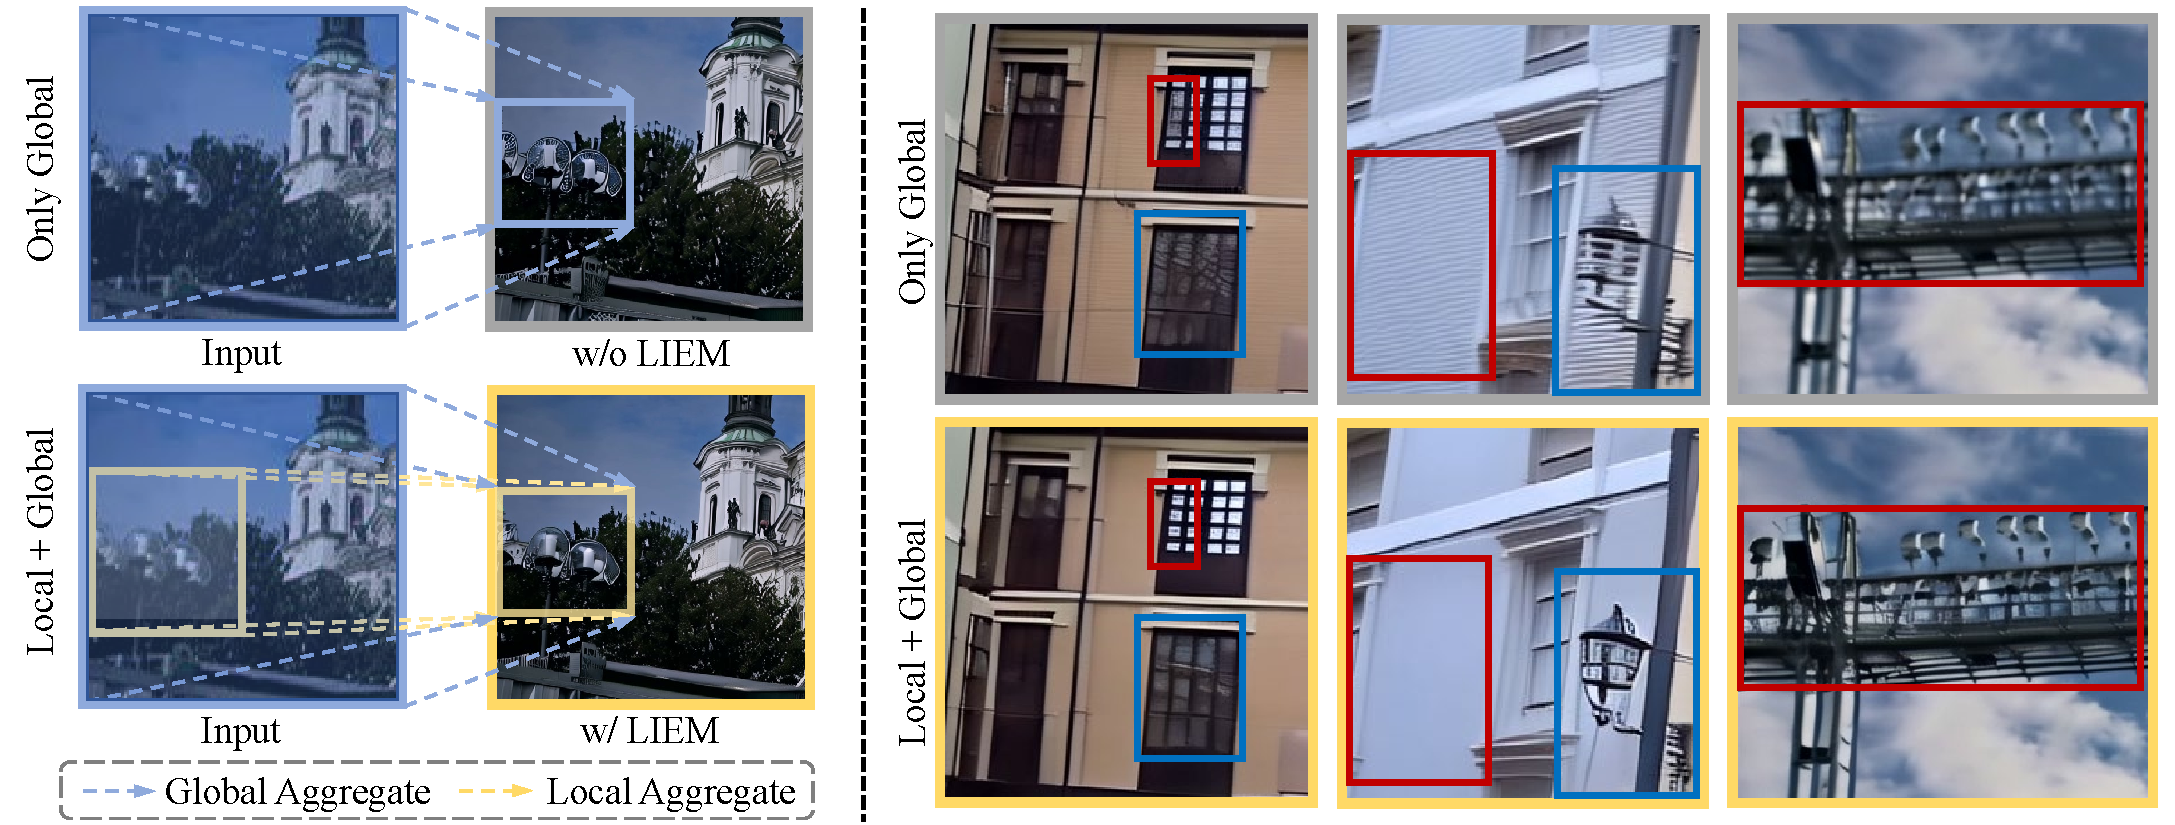
\includegraphics[width=0.98\linewidth]{figure/liem_motivation.pdf}\vspace{-2mm}
    \caption{\textbf{Motivation of LIEM.} \textbf{Left:} schematic diagram illustrating the impact of using only global structure versus a combination of local and global structures. \textbf{Right:} visual comparison on real-world and synthetic videos. (\textbf{Zoom-in for best view})}
    \label{motivation:liem}
\end{figure*}

\begin{figure*}[t!]
    \centering
    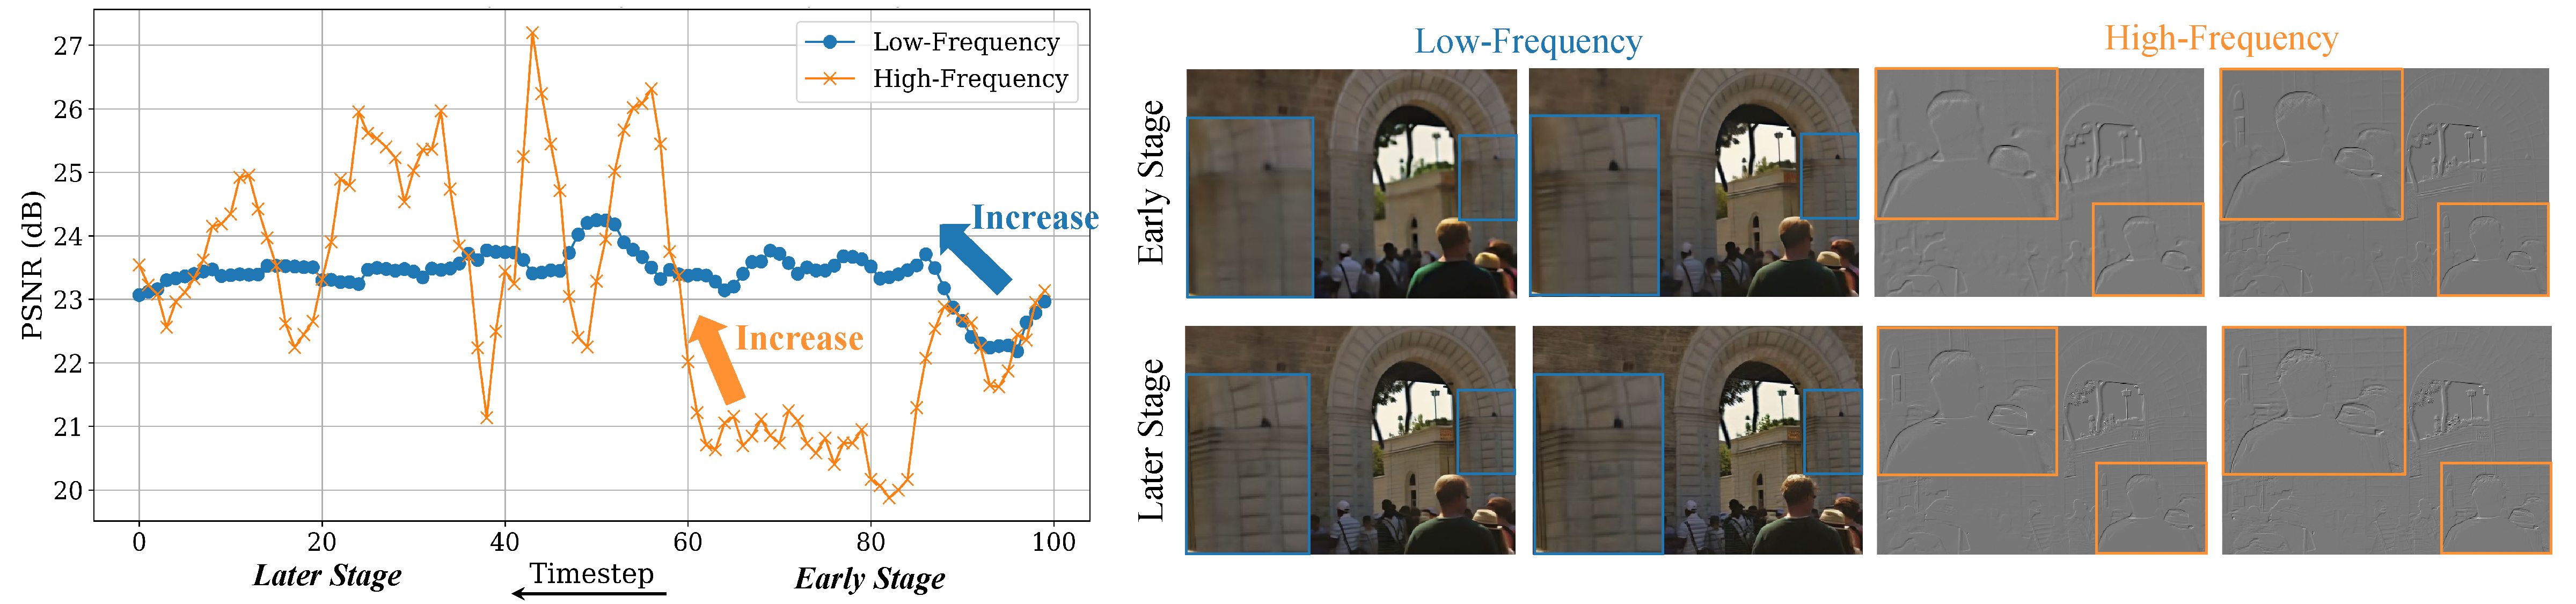
\includegraphics[width=1\linewidth]{figure/daf_motivation.pdf}
    \caption{\textbf{Motivation of DF Loss.} \textbf{Left}: PSNR curves of low- and high-frequency components relative to ground truth across diffusion steps. The low-frequency PSNR increases during the early diffusion steps, while the high-frequency PSNR rises in the later diffusion steps. 
    \textbf{Right}: visual results of low- and high-frequency components at different diffusion stage. (\textbf{Zoom-in for best view})}
    \label{motivation:daf}
\end{figure*}

\subsection{Overview}
\label{subsec:overview}

\paragraph{Modules.}
% \textbf{Modules.}
The~\name~primarily includes four modules: VAE \cite{kingma2013auto}, text encoder \cite{radford2021learning, raffel2020exploring}, ControlNet \cite{zhang2023adding} and T2V model \cite{zhang2023i2vgen, yang2024cogvideox} with Local Information Enhancement Module (\textbf{LIEM}) to alleviate the artifacts (further analysis is provided in Sec.~\ref{subsec:LIEM}). 
As depicted in Figure~\ref{fig:overview}, the VAE encoder takes HR videos $X_H$ and LR videos $X_L$ as input to generate latent tensors $Z_H$ and $Z_L$, respectively. The text encoder is responsible for generating text embeddings $c_{text}$ to provide high-level information. ControlNet takes $Z_L$ and $c_{text}$ as input to guide the T2V model output. Finally, the T2V model $\phi_\theta$ with \textbf{LIEM} receives noisy input $Z_t = \alpha_t Z_H + \sigma_t \epsilon$ ($t$ denotes diffusion step, $\alpha_t$ and $\sigma_t$ are noise scheduler parameters), $c_{text}$ and the control signal from ControlNet $c_{l}$ to predict the velocity $v_t \equiv \alpha_t \epsilon - \sigma_t Z_H$ \cite{salimans2022progressive}. 

\vspace{-1em}
\paragraph{Losses.}
% \noindent
% \textbf{Losses.}
We utilize v-prediction objective in optimization:
\begin{equation}
    \mathcal{L}_{v} = \mathbb{E}[\| v_t - \phi_\theta(Z_t, c_{text}, c_{l}, t) \|_2^2].
\end{equation}
%Due to the strong generalization ability of T2V models, using only the v-prediction objective for optimization may result in restored outputs with low fidelity, which is critical for video super-resolution tasks. To address this issue, we propose Dynamic Frequency (\textbf{DF}) Loss, which dynamically adjusts the constraint degree on the high-frequency and low-frequency components of the predicted $\hat{X}_H$ across different diffusion steps. The overall optimization objective for~\name~is as follows:
%
Given the strong generalization ability of T2V models, relying solely on the v-prediction objective for optimization may lead to restored outputs with low fidelity, an essential factor in video super-resolution tasks. 
To address this, we introduce Dynamic Frequency (\textbf{DF}) Loss, which adaptively adjusts the constraint on high- and low-frequency components of the predicted $\hat{X}_H$ across different diffusion steps. 
The overall optimization objective for~\name~is as follows:
%
\begin{equation}
    \mathcal{L}_{total} = \mathcal{L}_{v} + b(t)\mathcal{L}_{DF}(\hat{X}_H, X_H),
\end{equation}
where $b(t)= 1 - \frac{t}{t_{max}}$ is a weighting function ($t_{max}$ is set to 999) to balance $\mathcal{L}_{v}$ and $\mathcal{L}_{DF}$. 
With the proposed LIEM and DF loss,~\name~achieves high spatio-temporal quality, reduced artifacts and enhanced fidelity.

\subsection{Local Information Enhancement Module}
\label{subsec:LIEM}

\paragraph{Motivation.} 
% \noindent
% \textbf{Motivation.}
%Most T2V models primarily employ global attention mechanism \cite{liu2021global}, which is well-suited for the text-to-video task. This design choice aligns with the need to generate entire videos from scratch, capturing the global information. However, this approach may not be optimal for real-world video super-resolution, where complex degradations exist and local details are also important \cite{kong2022residuallocalfeaturenetwork}.
%
Most T2V models primarily use a global attention mechanism~\cite{liu2021global}, which is well-suited to text-to-video tasks by capturing global information to generate complete videos from scratch. 
However, this approach may be suboptimal for real-world video super-resolution, where complex degradations occur and local details are crucial~\cite{kong2022residual}.
%
Relying solely on global attention mechanisms presents two drawbacks for real-world video super-resolution: 
$1$) It \textit{complicates degradation removal}, as it processes the entire degraded video at once (the first and second columns in Figure~\ref{motivation:liem} (right)).
$2$) It \textit{lacks local details}, resulting in blurry outputs (the third column in Figure~\ref{motivation:liem} (right)). 

%As shown in Figure~\ref{motivation:liem}, when only using global attention mechanisms, there are two disadvantages for real-world video super-resolution: 1) It increases the difficulty of removing degradations since it handles the entire degraded video (\textit{e.g.,} see the first and second column of Fig. \ref{motivation:liem} (right)). 2) It lacks local information, leading to blurry results (\textit{e.g.,} see the third column of Figure~\ref{motivation:liem} (right)). 

\vspace{-1em}
\paragraph{Details of LIEM.}
% \noindent
% \textbf{Details of LIEM.}
To address the above issues, we propose a simple but effective approach: adding a \textit{Local Information Enhancement Module} (LIEM) before the global attention block to make T2V model pay more attention to local information. It can be expressed by:
% To address these issues, we propose a simple yet effective approach that integrates a LIEM before the global attention block to encourage the T2V model to better capture local details: %. This can be expressed as:
\begin{equation}
    L(F_I) = Sigmoid(Conv_{3\times3}(Concat(AP(F_I), MP(F_I)))),
\end{equation}
\begin{equation}
    F_O = G(L(F_I) \cdot F_I) + F_I,
\end{equation}
where $AP(\cdot)$ and $MP(\cdot)$ denote average pooling and max pooling, respectively. $F_I$ and $F_O$ represent the input and output features, while $G(\cdot)$ and $L(\cdot)$ refer to the global attention block and LIEM. We adopt the local attention block in CBAM \cite{woo2018cbam} as LIEM for simplicity. 
Additional analysis on the impact of adding LIEM is provided in Sec.~\ref{sec:liem_ablation}.
%
%where $AP(\cdot)$ and $MP(\cdot)$ denote average pooling and max pooling, respectively. $F_I$ and $F_O$ represent the input and output features, while $G(\cdot)$ and $L(\cdot)$ refer to the global attention block and LIEM. As the design of LIEM is not central to our~\name~ approach, we adopt the local attention block from CBAM \cite{woo2018cbam} for simplicity. Additional analysis on the impact of LIEM is provided in
%
Intuitively, as shown in the second row of Figure~\ref{motivation:liem} (left), %with LIEM, the T2V model can first deal with local region degradation and then aggregate global features, reducing the difficulty of degradation removal and alleviating generated artifacts. 
incorporating LIEM enables the T2V model to address local region degradation first and then aggregate global features. 
This approach reduces the complexity of degradation removal and mitigates artifacts. 
Furthermore, the T2V model with LIEM produces clearer, more detailed results due to the enriched local information.
 
\subsection{Dynamic Frequency Loss}
\label{subsec:daf}


\begin{table*}[t!]
    \caption{Quantitative evaluations on diverse VSR benchmarks from synthetic (UDM10, REDS30, OpenVid30) and real-world (VideoLQ) sources. The best performance is highlighted in \textbf{bold}, and the second-best in \underline{underlined}. E$^*_{warp}$ refers to E$_{warp}$ ($\times10^{-3}$).} \label{tab:my_label}
    \centering
    \resizebox{\textwidth}{!}{
    \begin{tabular}{cc|cccc|cccccc}
    \hline
    \multirow{2}{*}{Datasets} & \multirow{2}{*}{Metrics} & Real-ESRGAN & DBVSR & RealBasicVSR & RealViformer & ResShift & StableSR & Upscale-A-Video & MGLDVSR & Ours \\ 
    ~ & ~ & ICCVW 2021 & ICCV 2021 & CVPR 2022 & ECCV 2024 & NeurIPS 2023 & IJCV 2024 & CVPR 2024 & ECCV 2024 & - \\ \hline \hline
    \multirow{5}{*}{UDM10} & PSNR$\uparrow$ & 22.41 & 19.65 & 23.64 & \textbf{24.00} & 22.90 & 23.50 & 21.29 & 23.74 & \underline{23.91} \\
    ~ & SSIM$\uparrow$ & 0.6476 & 0.4747 & 0.6842 & \underline{0.6896} & 0.5451 & 0.6599 & 0.5967 & 0.6826 & \textbf{0.7164} \\
    ~ & LPIPS$\downarrow$ & 0.2769 & 0.4566 & 0.2514 & 0.2325 & 0.4036 & 0.2785 & 0.3006 & \underline{0.2195} & \textbf{0.1885} \\
    ~ & DOVER$\uparrow$ & 0.4831 & 0.0959 & 0.5039 & 0.5055 & 0.3252 & 0.3490 & \underline{0.5309} & 0.4896 & \textbf{0.5422} \\
    ~ & E$^*_{warp}$ $\downarrow$ & 11.17 & 12.56 & 5.14 & 3.57 & 12.69 & 8.89 & \underline{2.83} & 6.03 & \textbf{2.68} \\ \hline
    \multirow{5}{*}{REDS30} & PSNR$\uparrow$ & 19.56 & 14.85 & \underline{20.85} & \textbf{20.86} & 19.93 & 20.32 & 19.71 & 20.57 & 20.29 \\
    ~ & SSIM$\uparrow$ & 0.4862 & 0.2941 & \textbf{0.5469} & 0.5377 & 0.4261 & 0.5043 & 0.4315 & 0.5113 & \underline{0.5411} \\
    ~ & LPIPS$\downarrow$ & 0.3376 & 0.5915 & 0.2899 & \underline{0.2597} & 0.4422 & 0.3857 & 0.3443 & \textbf{0.2240} & 0.2804 \\
    ~ & DOVER$\uparrow$ & 0.3182 & 0.0600 & 0.3483 & 0.3400 & 0.2221 & 0.2519 & 0.2857 & \underline{0.3857} & \textbf{0.4017} \\
    ~ & E$^*_{warp}$ $\downarrow$ & 19.1 & 18.00 & 8.32 & \textbf{6.06} & 17.40 & 22.14 & 15.65 & 12.28 & \underline{7.30} \\ \hline
    \multirow{5}{*}{OpenVid30} & PSNR$\uparrow$ & 24.62 & 21.14 & 24.63 & \textbf{26.21} & 24.29 & 24.91 & 24.41 & 24.73 & \underline{25.30} \\
    ~ & SSIM$\uparrow$ & 0.7778 & 0.5887 & 0.7759 & \underline{0.8080} & 0.6070 & 0.7633 & 0.7167 & 0.7686 & \textbf{0.8371} \\
    ~ & LPIPS$\downarrow$ & 0.1994 & 0.4207 & 0.2297 & \underline{0.1881} & 0.3902 & 0.2102 & 0.2479 & 0.2074 & \textbf{0.1011} \\
    ~ & DOVER$\uparrow$ & 0.6992 & 0.1819 & \underline{0.7345} & 0.7275 & 0.5435 & 0.6368 & 0.7201 & 0.7191 & \textbf{0.7393} \\
    ~ & E$^*_{warp}$ $\downarrow$ & 8.46 & 12.11 & 4.12 & \underline{2.52} & 9.78 & 8.87 & 4.72 & 4.82 & \textbf{1.82} \\ \hline \hline
    \multirow{4}{*}{VideoLQ} & ILNIQE$\downarrow$ & 27.95 & 27.19 & 26.29 & 26.11 & 25.92 & 29.97 & \underline{24.49} & \textbf{23.94} & 25.35 \\
    ~ & DOVER$\uparrow$ & 0.4967 & 0.3392 & \underline{0.5285} & 0.4804 & 0.4113 & 0.4775 & 0.4833 & 0.5319 & \textbf{0.5431} \\
    ~ & E$^*_{warp}$ $\downarrow$ & 8.00 & 7.75 & 6.52 & \textbf{5.10} & 8.33 & 9.26 & 10.89 & 7.82 & \underline{6.38} \\ \hline
    \end{tabular}}
\end{table*}




\paragraph{Motivation.}
% \textbf{Motivation.}
%Due to the powerful generative ability of pre-trained diffusion models, the restored results may produce elements that do not align with the ground truth, thereby compromising fidelity \cite{wu2024seesr, yu2024scaling}. As shown in Fig. \ref{motivation:daf} (Right), we observed an interesting pattern while examining the restored results at each diffusion step: in the early stages, the diffusion model primarily reconstructs the structure rather than the details, whereas in the later stages, once the structure is largely complete, the focus shifts to reconstructing the details. To further demonstrate this phenomenon, we present the PSNR curves of low-frequency and high-frequency components with respect to the ground truth as the diffusion steps change, as shown in Fig. \ref{motivation:daf} (Left). The low-frequency PSNR increases in the early stages, while the high-frequency PSNR increases in the later stages, which is consistent with the visualization results.
The powerful generative capacity of diffusion models may compromise the fidelity in restored result~\cite{wu2024seesr, yu2024scaling}. 
In Figure~\ref{motivation:daf} (Right), an interesting pattern emerges when examining restored results at each diffusion step during inference. 
In the early stages, the model primarily reconstructs structure with low frequency, whereas in later stages, after the structure is largely complete, focus shifts to refining details with high frequency. 
To further illustrate this phenomenon, Figure~\ref{motivation:daf} (Left) presents PSNR curves of low- and high-frequency components against the ground truth across diffusion steps. 
The low-frequency PSNR rises in the early stages, while the high-frequency PSNR increases later, aligning with the visual results.

%Fidelity can be divided into two classes: 1) low-frequency fidelity, such as large structures and instances. 2) high-frequency fidelity, such as edges and textures, which correspond to the characteristics of the denoising process. This raises the question: can we design a loss function that utilizes this characteristic to decouple fidelity, thereby reducing optimization difficulty? Specifically, we aim to constrain the model to pay more attention to the low-frequency components in the early stages and focus on high-frequency components in the later stages.

Fidelity can be divided into two types: 
$1$) Low-frequency fidelity, encompassing large structures and instances. 
2) High-frequency fidelity, including edges and textures, aligning with the characteristics of the denoising process. 
This raises a question: Can we design a loss function that exploits this characteristic to decouple fidelity and simplify optimization?
Specifically, we aim to guide the model to \textit{prioritize low-frequency components in the early stages}, shifting focus to \textit{high-frequency components later}.

\begin{figure}[t!]
    \centering
    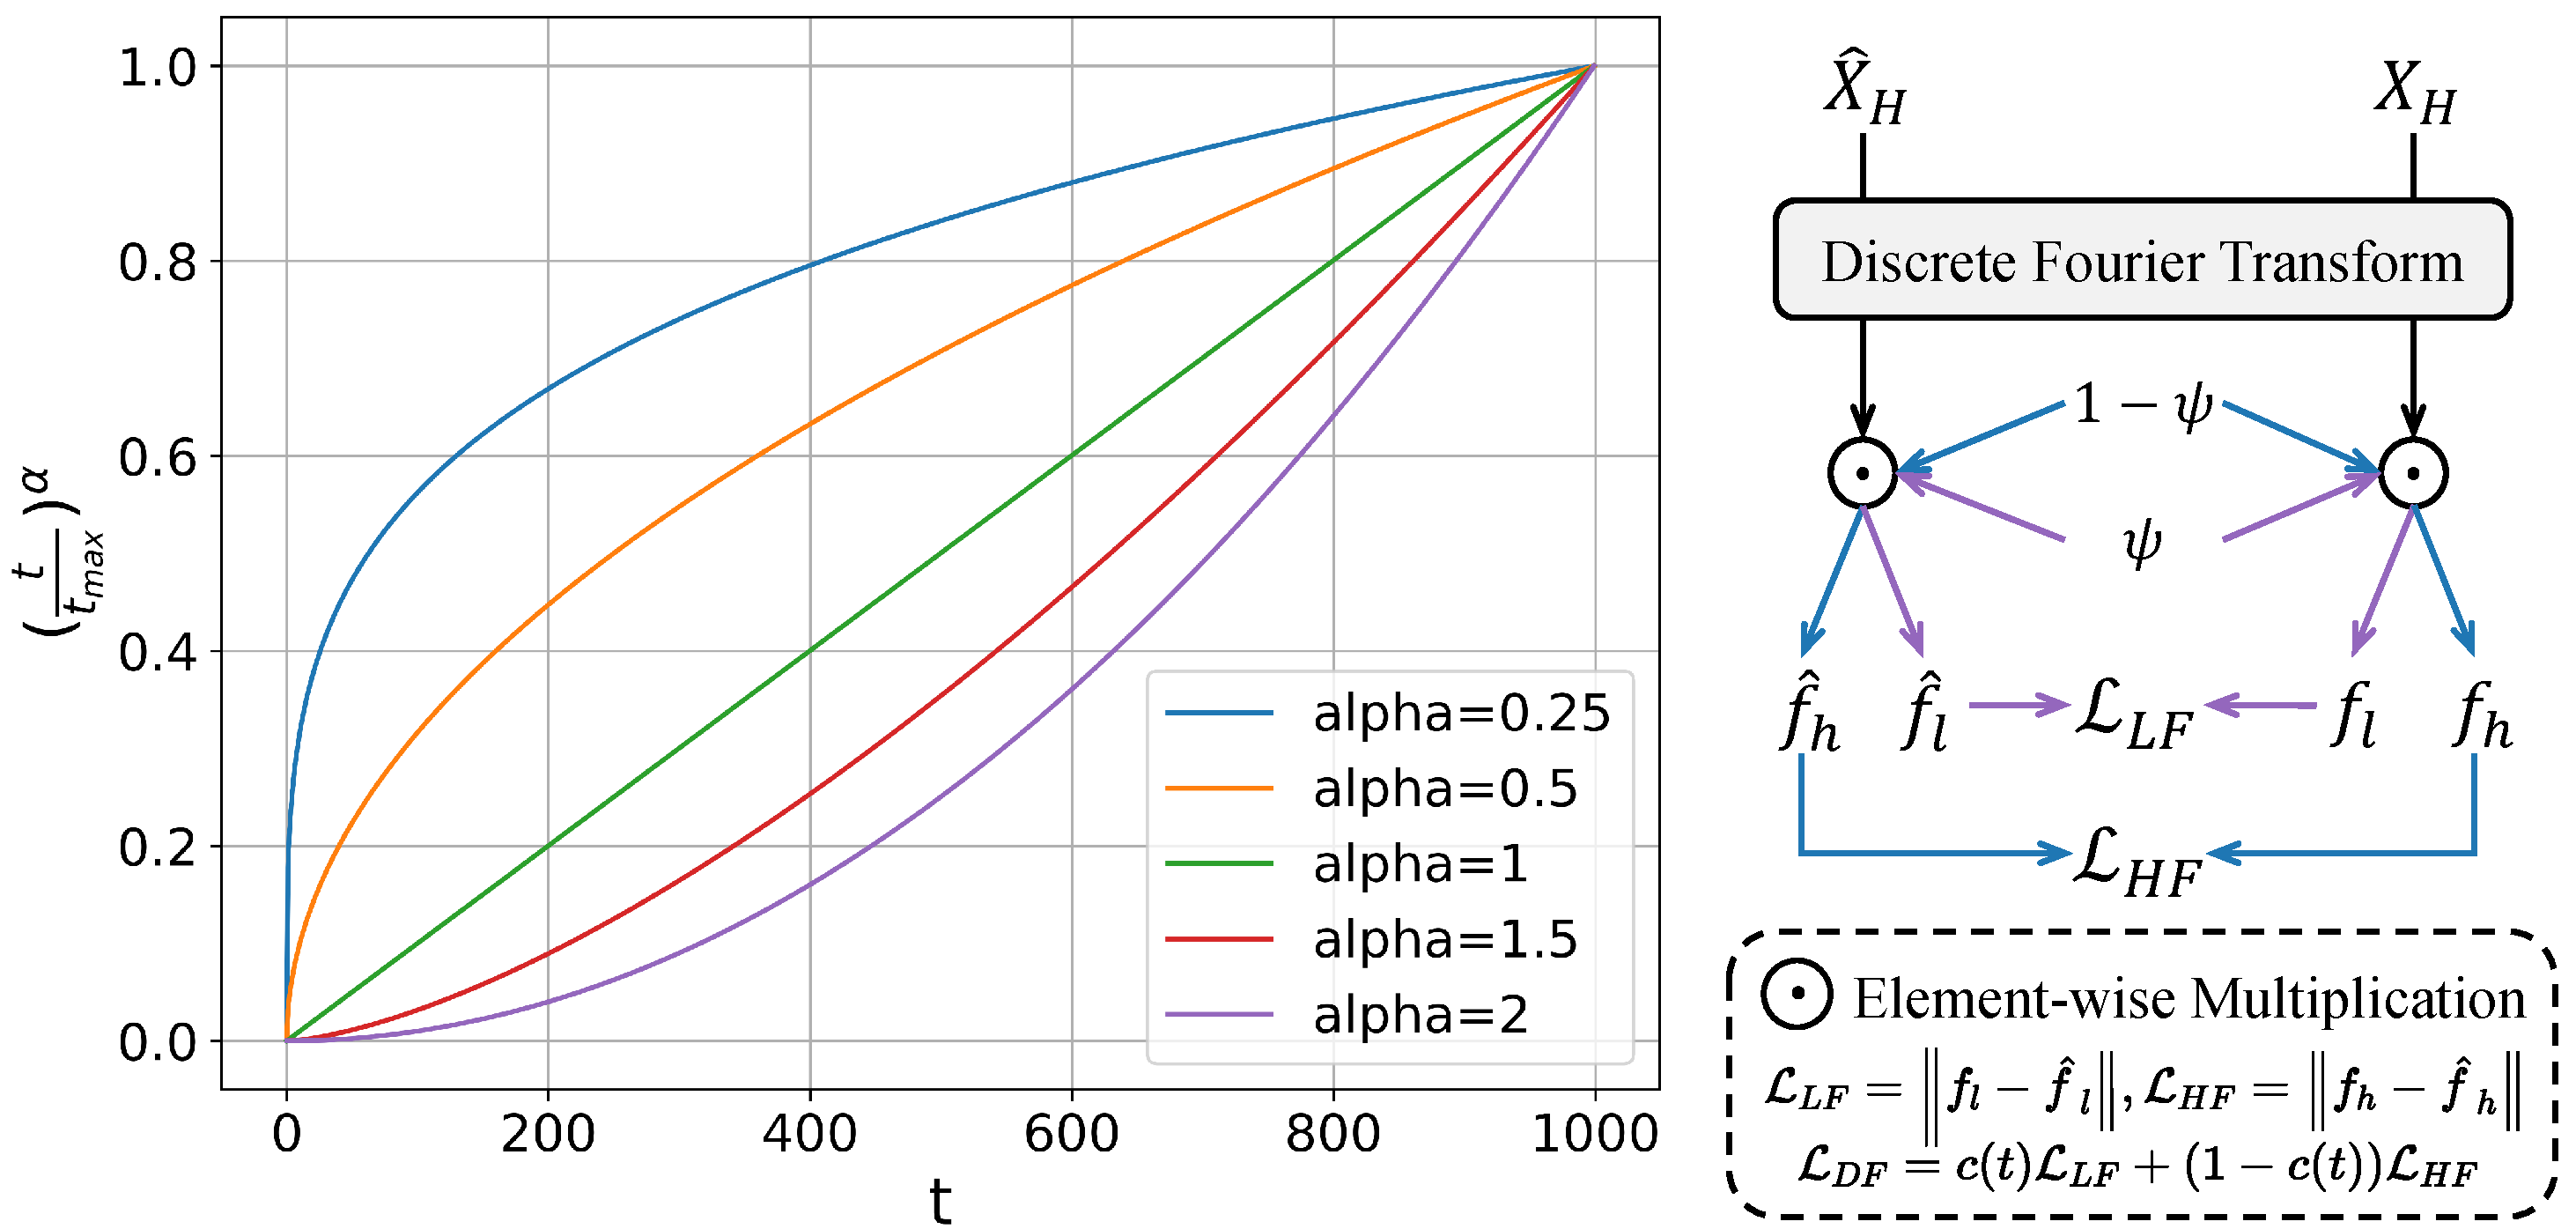
\includegraphics[width=1\linewidth]{figure/daf_method.pdf}
    \caption{\textbf{Dynamic Frequency Loss.} \textbf{Left}: curves of weighting function $c(t)$ for different $\alpha$. \textbf{Right}: details of DF loss.}
    \label{fig:daf_method}
\end{figure}

\vspace{-1em}
\paragraph{Details of DF Loss.}
% \noindent
% \textbf{Details of DF Loss.}
Here, we propose Dynamic Frequency Loss. 
Specifically, in each diffusion step $t$, we use the following equation to obtain the estimated $\hat{Z}_H$:
\begin{equation}
    \hat{Z}_H = \sigma_t^{-1}(\alpha_t\epsilon-\phi_\theta(Z_t, c_{text}, c_{l}, t)).
\end{equation}
Then, we use the decoder to convert the latent $\hat{Z}_H$ back to the pixel space, resulting in $\hat{X}_H$. After that, we apply Discrete Fourier Transform (DFT) to transform $\hat{X}_H$ into the frequency domain as shown in Figure~\ref{fig:daf_method}. 
We predefine a low-frequency pass filter $\psi$ to obtain the low- and high-frequency: %The process can be formulated below:
% Instead of using a predefined filter to separate the low- and high-frequency components, we propose a learnable adaptive filter $\psi_{\theta'}$ that takes the diffusion step $t$ and the HR video $X_H$ as inputs. The process can be formulated below:
\begin{equation}
    \hat{f}_l = \mathcal{F}(\hat{X}_H) \odot \psi, \hat{f}_h = \mathcal{F}(\hat{X}_H) \odot (1-\psi),
\end{equation}
where $\mathcal{F}(\cdot)$ is DFT, $\odot$ is element-wise multiplication. $\hat{f}_{l}$ and $\hat{f}_{h}$ denote the low and high frequency of $\hat{X}_H$. The proposed DF loss can be written as: 
\begin{equation}
    \mathcal{L}_{LF} = \| f_l - \hat{f}_l \|, \mathcal{L}_{HF} = \| f_h - \hat{f}_h \|,
\end{equation}
\begin{equation}
    \mathcal{L}_{DF} = c(t)\mathcal{L}_{LF} + (1-c(t))\mathcal{L}_{HF},
\end{equation}
where $f_l$ / $f_h$ stand for low- / high-frequency of $X_H$, respectively. $c(t) = (t/t_{max})^\alpha$ is the weighting function.
%
% --- inline annotations
%
\newcommand{\red}[1]{{\color{red}#1}}
\newcommand{\todo}[1]{{\color{red}#1}}
\newcommand{\TODO}[1]{\textbf{\color{red}[TODO: #1]}}
% --- disable by uncommenting  
% \renewcommand{\TODO}[1]{}
% \renewcommand{\todo}[1]{#1}

\usepackage{xcolor}
\usepackage{graphicx}
\usepackage{booktabs}
\usepackage{amsmath} 
\usepackage{amsfonts}
\usepackage{amssymb}
\usepackage{multirow} 
\usepackage{makecell}
\newcommand{\shline}{\Xhline{1.1pt}} % Adjust thickness as desired

\section{Experiments}
\label{sec:experiments}

We present results for supervised video classification and self-supervised masked auto-encoding with frozen representations evaluated on two downstream tasks: video classification and point tracking. To analyse the memory capabilities of our model, we also include a reconstruction task of frames seen in the distant past. Using the same task, we study the generalisation capabilities to longer sequences than seen during training. We follow the ViT scaling configurations and, unless otherwise stated, we use the \textbf{B}ase version for our model for all our experiments. We specify the number of parameters for all models considered in our experiments, and we include in the supplementary material all the training hyperparameters and data augmentations used in all experiments.

\subsection{Supervised video classification}

\par \noindent \textbf{Datasets:}
We use large-scale real-world datasets for the supervised video classification task. Kinetics400~\citep{Carreira_2017_CVPR} contains 241,512 videos\footnote{Kinetics is a dynamic dataset (videos may be removed from
YouTube). Our current version has 241,512 videos, compared to 267,000 videos reported in~\cite{vivit}, so a decrease of almost 10\%, noticeable in the final performance.} across train, validation, and test splits, 10s-long (25fps), spanning 400 classes. This dataset is known to require modelling appearance for successful action recognition. To challenge our model's capability of understanding motion, we also use SSv2 dataset~\citep{goyal2017something}, which contains 220,847 shorter videos (2-6s long), sampled at 12fps, representing 174 classes. This dataset includes actions that differ in finer motion-related details, requiring a deeper temporal understanding, e.g. \textit{pouring something into something} vs \textit{pretending to pour something into something}. 

\par \noindent \textbf{Baselines:}
We use ViViT~\citep{vivit} as our main baseline. We consider the full self-attention version, which patchifies and flattens the entire video, prepends a video class token, then runs self-attention blocks. We also consider the factorised encoder version (ViViT FE), which runs a ViT image model over all the frames, and uses temporal self-attention blocks to integrate the information over time. Finally, we also consider a baseline that uses only LRU recurrent and MLP blocks, configured similar to VideoMamba~\cite{li2024videomambastatespacemodel}, i.e. it does not use self-attention blocks, denoted \textit{PureLRU}. Similar to ViViT, this model first patchifies and flattens the video, prepends a class token, then applies a sequence of recurrent blocks. All baselines use learnt spatio-temporal positional encoding, whereas the proposed \ssm\ uses only spatial positional encoding as the temporal dimension is implicitly modelled through its recurrence.


\par \noindent \textbf{Results:} We include results for training from scratch or using Imagenet pre-trained weights to initialise the weights of the ViT blocks. Figure~\ref{fig:baselines} shows a first comparison between \ssm\ and the above baselines, with all models being trained from scratch on supervised classification on SSv2. We consider the \textbf{S}mall version for all models as the larger \textbf{B}ase version shows stability issues when trained from scratch, as reported in other works as well~\cite{li2024videomambastatespacemodel,vivit}. As expected, the performance on this challenging dataset when training from scratch is far from SOTA, but it clearly shows that the proposed factorisation has superior video modelling capabilities compared to baselines, ViViT-S with full self-attention being the closest competitor. PureLRU's performance is very poor, which is in line with the findings of other works (\eg VideoMamba) who report that bidirectional (non-causal) processing of the input is needed for good performance. 

We report further results comparing against ViViT-B and ViViT-L with full self-attention when using Imagenet pre-trained weights; see Table~\ref{tab:ssv2} for SSv2 results and Table~\ref{tab:kinetics} for Kinetics400 results.
We can observe that our model achieves better performance compared to ViViT baselines on SSv2, but it is slightly below ViViT-L on Kinetics400. This result could reflect the difference between the two datasets mentioned above: outperforming ViViT-L on SSv2 suggests that \ssm\ is superior at modelling motion compared to ViViT, but on Kinetics where the appearance is enough for successful classification, both models are on par. We consider this to be a strong positive result for our model given that it has about 3x less parameters compared to ViViT-L and significantly lower FLOPs count and memory footprint as shown in Figure~\ref{fig:memory}.

\begin{figure}[t]
  \centering
  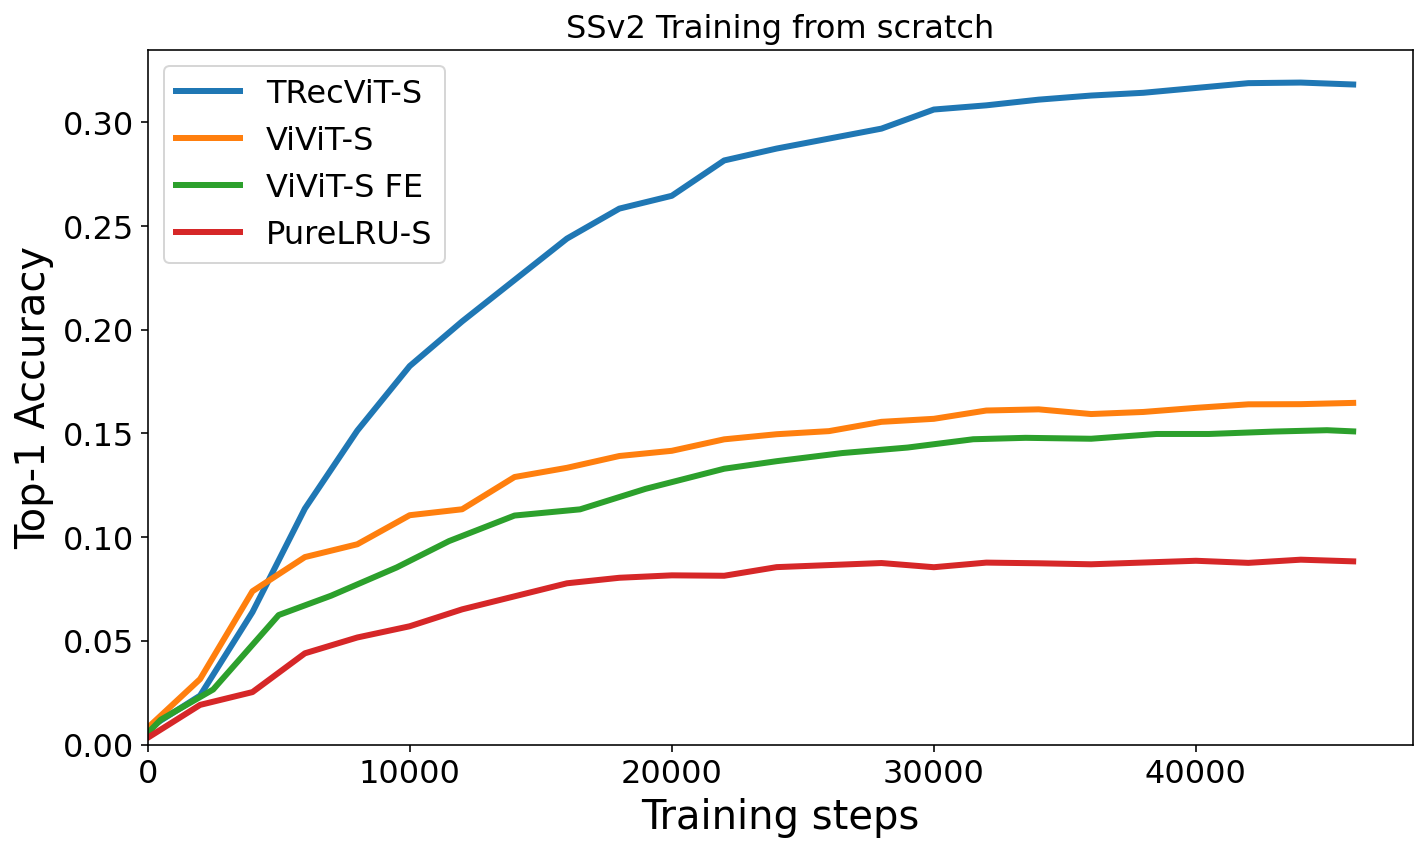
\includegraphics[width=.9\linewidth]{img/scratch.png}
  \caption{\ssm\ compared to baselines on supervised video classification on SSv2 dataset, trained from scratch. The plot shows the evolution of the evaluation accuracy as training progresses.
  }

  \label{fig:baselines}
\end{figure}
 

 \begin{figure*}[h]
  \centering
  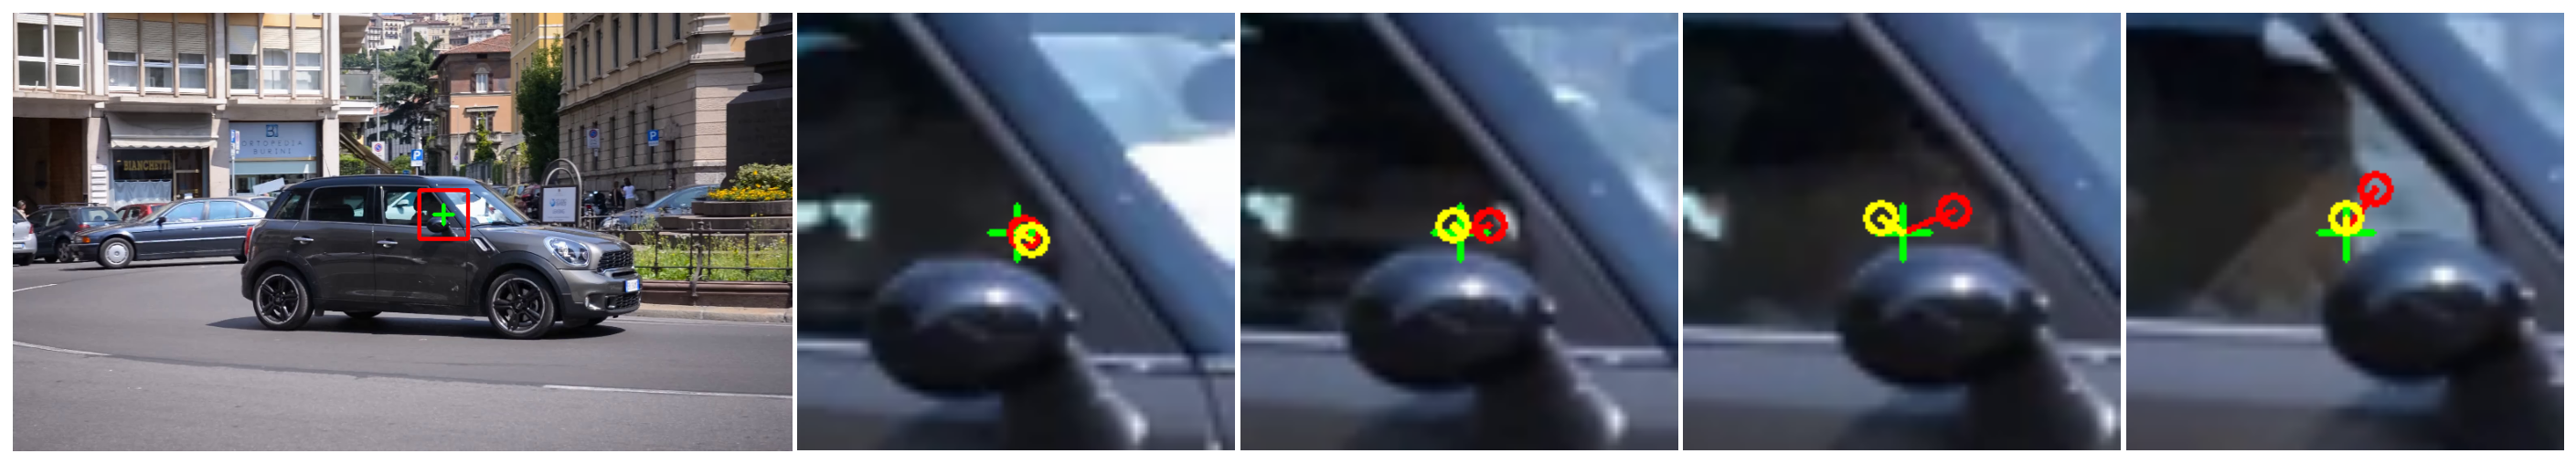
\includegraphics[width=\linewidth]{img/davis.png}
  \caption{Qualitative results obtained by \ssm\ for point tracking on DAVIS dataset compared to VideoMAE. The leftmost image indicates the point to track in the original frame, and the images towards the right show zoom-ins on subsequent frames. Green plus (+) marker indicates the ground truth, yellow circle indicates \ssm's predictions and red circles indicate VideoMAE's predictions.}
  \label{fig:tracking}
\end{figure*}


\begin{table}
    \centering
    \small{
    \begin{tabular}{l|c|c|r}
    \hline
    \textbf{Model} & \textbf{Patch size} & \textbf{Top-1 acc (\%)} & \textbf{\# params} \\
    \hline
    ViViT-B & (2, 16, 16) & 59.1 & 90M \\
    ViViT-L & (2, 16, 16) & 65.9 & 320M \\
    \ssm\ & (1, 16, 16) & \textbf{66.8} & 109M\\
    \hline
    \end{tabular}}
    \caption{Performance of \ssm\ compared to ViViT-B and ViViT-L baselines on SSv2 dataset with all models initialised from Imagenet pre-training. For ViViT-L, we use the result reported by its authors, for ViViT-B we obtained the results internally as they were not reported in the original paper for this dataset.}
    \label{tab:ssv2}
    \end{table}
    
\begin{table}
    \centering
    \small{
    \begin{tabular}{l|c|c|r}
    \hline
    \textbf{Model} & \textbf{Patch size} & \textbf{Top-1 acc (\%)} & \textbf{\# params} \\
    \hline
    ViViT-B & (2, 16, 16) & 78.1 & 90M \\
    ViViT-L & (2, 16, 16) & \textbf{78.7} & 320M \\
    \ssm\ & (1, 16, 16) & 78.4 & 109M\\
    \hline
    \end{tabular}}
    \caption{Performance of \ssm\ compared to ViViT-B and ViViT-L baselines on Kinetics400 dataset, with all models initialised from Imagenet pre-training. For ViViT-B and ViViT-L, we include the result we obtained internally by re-training the model on the current Kinetics400 dataset version; see footnote. In the original paper, the authors reported 80.3\% on Kinetics400 for ViViT-L.}
    \label{tab:kinetics}
    \end{table}

\subsection{Self-supervised masked autoencoding}
\label{sec:mae}
We use Kinetics400 for self-supervised pre-training from scratch and we report results on multiple downstream datasets and tasks by fine-tuning attention readout heads on top of frozen representations. We choose this setup, as opposed to fine-tuning end-to-end, as the  performance in this case more clearly reflects the quality of the pre-trained representations. As mentioned in the previous section, we use a large masking ratio (0.90), which makes pre-training very efficient. We report the number of parameters for every model considered. Note that the number of parameters for \ssm\ is different from the one reported in the previous section due to the addition of the readout heads.

\par \noindent \textbf{Video classification:}  We report video classification accuracy as downstream task using attention readout heads on SSv2 and Kinetics400. We compare the performance against VideoMAE-L~\cite{tong2022videomae} in Table~\ref{tab:selfsup}. Our model obtains slightly better performance on both datasets compared to this strong baseline, despite having almost 3$\times$ less parameters. 

\par \noindent \textbf{Point tracking:} To demonstrate that our model can handle dense(r) tasks as well, we evaluate the same frozen MAE representations for the point tracking task. We use the recurrent architecture in MooG~\cite{steenkiste2024moving} as a readout due to its simplicity. MooG uses light cross-attention layers to process the embeddings of each frame in order, and the readout state is carried over through time. We finetune the MooG readout head using MOVi-E dataset~\cite{movie} as done in popular point tracking works~\cite{DoerschYVG0ACZ23}. We evaluate these fine-tuned representations on two datasets: Perception Test~\citep{patraucean2023perception} and DAVIS dataset~\cite{davis2017} with point tracks extracted in~\cite{doersch2022tapvid}. We report average Jaccard metric~\cite{doersch2022tapvid} for \ssm\ compared with MooG and VideoMAE; see Table~\ref{tab:pt}. \ssm\ obtains better performance on both datasets compared to baselines, which reinforces the observation that our proposed model has strong motion modelling capabilities. We include qualitative results for this task in Figure~\ref{fig:tracking}. We can observe that the results are visibly better compared to VideoMAE. More visualisations are included in the supplementary material.

\begin{table}
    \centering
    \small{
    \begin{tabular}{l|c|c|r}
    \hline
    \textbf{Model} & \textbf{Dataset} & \textbf{Top-1 acc (\%)} & \textbf{\# params} \\
    \hline
    VideoMAE & Kinetics400 & 45.8 & 330M \\
    \ssm\ & Kinetics400 & \textbf{46.0} & 128M\\
    \hline
    \hline
    VideoMAE & SSv2 &  53.7 & 330M \\
    \ssm\ & SSv2 &  \textbf{53.9} & 128M\\
    \hline
    \end{tabular}}
    \caption{Performance of \ssm\ compared to VideoMAE on video classification using frozen MAE representations, pre-trained on Kinetics400.}
    \label{tab:selfsup}
    \end{table}

\begin{table}
    \centering
    \small{
    \begin{tabular}{l|c|c|c|r}
    \hline
    \textbf{Model} & \textbf{Dataset} & \textbf{\# frames} & \textbf{AJ} & \textbf{\# params} \\
    \hline
    MooG & DAVIS & 8 & 0.687 & 35M \\
    VideoMAE & DAVIS & 8 & 0.703 & 330M \\
    \ssm\ & DAVIS & 8 & \textbf{0.706} & 128M\\
    
    \hline
    \hline
    MooG & Perception Test & 16 & 0.760 & 46.5M \\
    VideoMAE & Perception Test & 16 & 0.761 & 330M \\
    \ssm\ & Perception Test & 16 & \textbf{0.783} & 128M\\
    \hline
    \end{tabular}}
    \caption{Performance of \ssm\ compared to baselines on point tracking task on DAVIS and Perception Test datasets. All models use frozen representations evaluated using the readout head from MooG.}
    \label{tab:pt}
    \end{table}

\begin{figure*}[h]
  \centering
  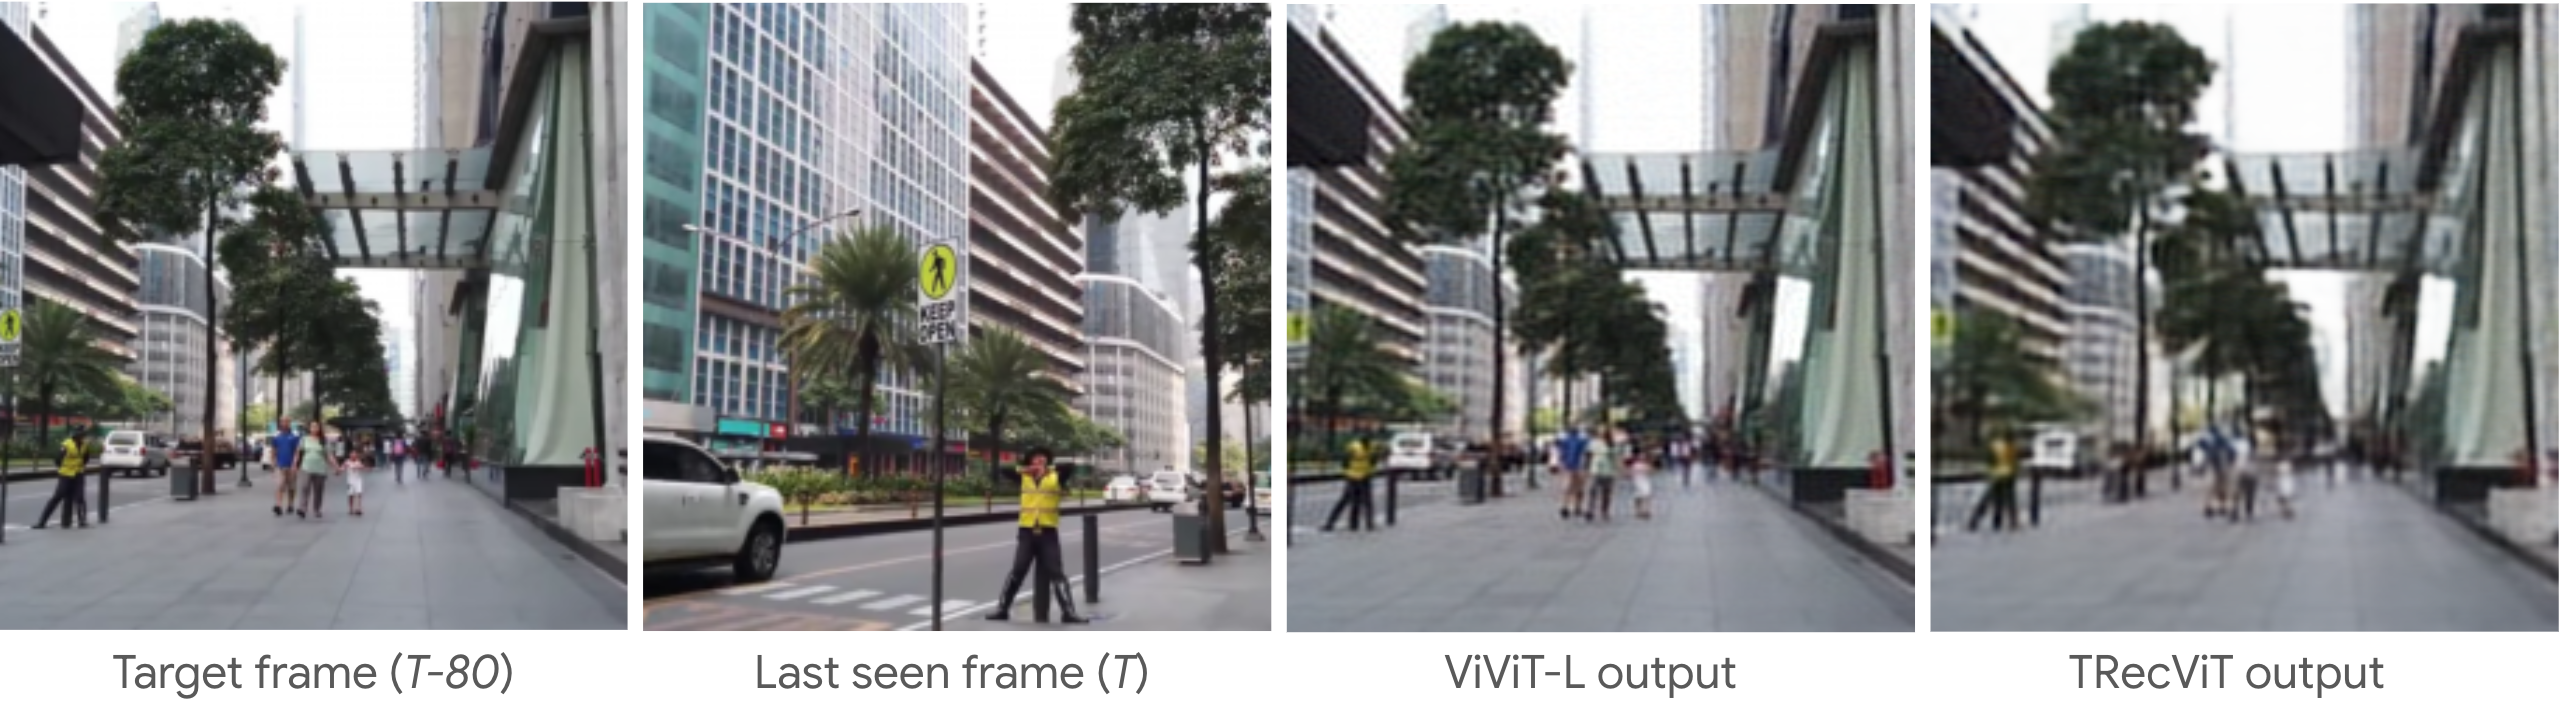
\includegraphics[width=\linewidth]{img/wtlong.png}
  \caption{Qualitative results obtained by \ssm\ on the dense memorisation task compared to ViViT-L. Both models are trained using Imagenet pre-trained weights, on video sequences of $T=64$ frames and they reconstruct the $(T-48)^\text{th}$ frame.}
  \label{fig:wt}
\end{figure*}

\begin{figure}[t]
\centering
\begin{subfigure}{0.48\linewidth}
    \centering
    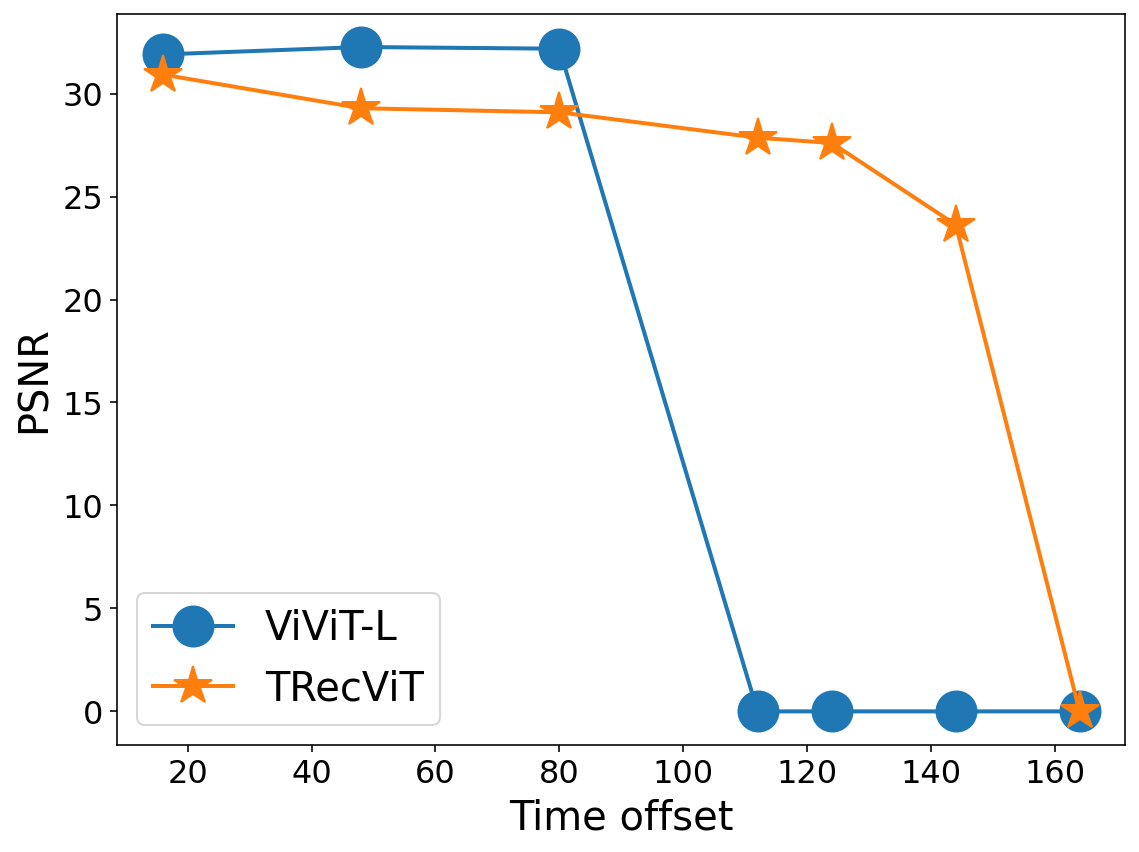
\includegraphics[width=\textwidth]{img/psnr.png}
    \caption{PSNR comparison}
\end{subfigure}%
\hfill
\begin{subfigure}{0.48\linewidth}
    \centering
    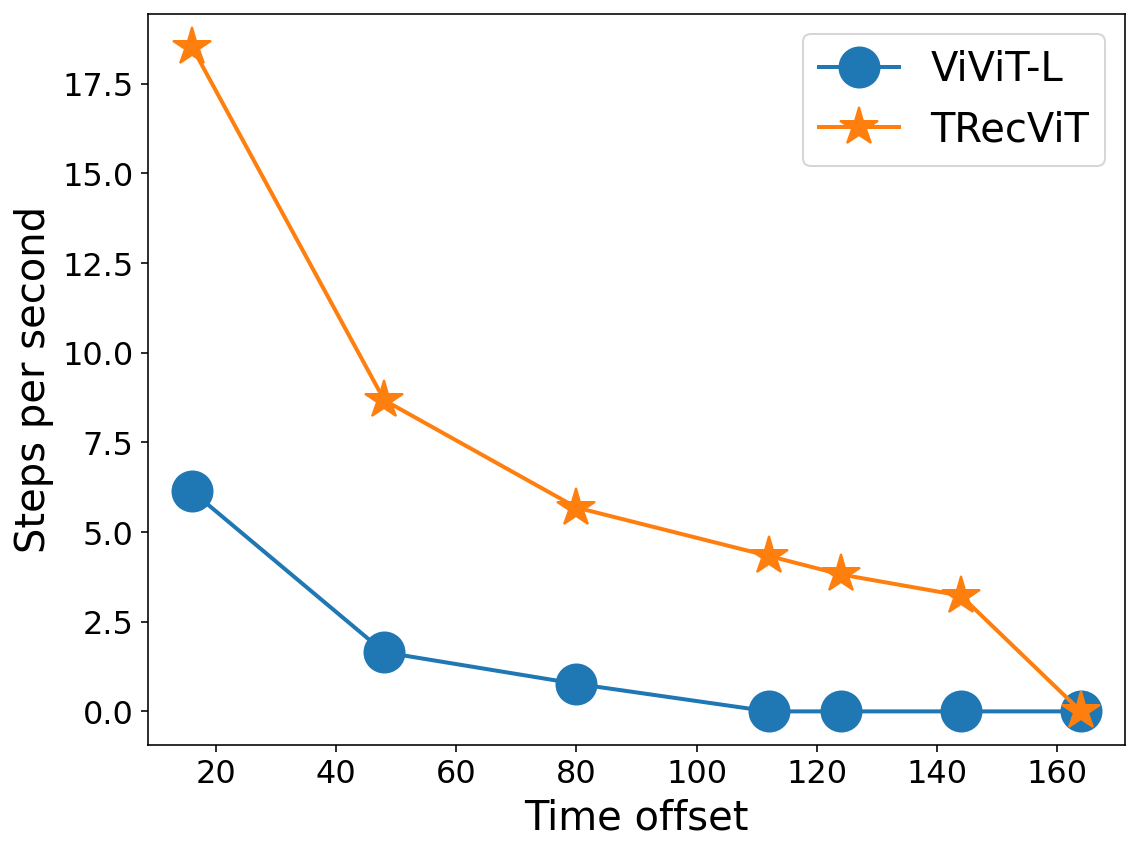
\includegraphics[width=\textwidth]{img/sps.png} 
    \caption{Steps-per-second comparison}
\end{subfigure}
\caption{Long video memorisation task. At time $T$, the model has to reconstruct the $(T-k)^\text{th}$ frame seen in the past. The plots show PSNR and throughput (steps-per-second) for increasing time offset $k$. For both models, the data points with $0$ value on the $y$-axis correspond to OOM.
}
\label{fig:psnr}
\end{figure}

\subsection{Long video memorisation task}
\label{sec:longtask}

Transformer models for language are known to be excellent at retrieving information from context, as they cache the keys and values for the entire history. On the other hand, LRUs / SSMs and RNNs in general struggle with such \emph{needle-in-the-haystack} style tasks as they need to perform the retrieval based on the compressed history kept in their recurrent state~\cite{jelassi2024repeat, de2024griffinmixinggatedlinear}. 
We are interested in studying this aspect in the video domain as well. We set up a simple reconstruction task where the model has to remember the frame seen at a given time-step in the past. For our analysis, we run multiple experiments where the model is tasked to reconstruct the $(T-k)^{\text{th}}$ frame from the past, with increasing value for $k\in\{16, 48, 80, 112, 144, 164\}$ frames. We employ Walking Tours dataset~\cite{venkataramanan2023imagenet}, which contains hour-long videos, and the scenery changes constantly, hence we are guaranteed that the video frames seen most recently will be very different compared to the frames seen earlier on. We scale the videos to $224\times224$ pixels. Again, we adopt ViViT-L as baseline, and we train both models using Imagenet pretrained weights. For ViViT-L, we keep all the outputs from all $T$ time steps and apply temporal pooling and a $1\times1$ convolution to get the expected shape for the reconstructed frame. For \ssm, we simply keep the output of the last layer at time step $T$ and reshape it to the expected shape. We show quantitative and qualitative results respectively in Figures~\ref{fig:psnr} and~\ref{fig:wt}. We can observe that there is a performance--efficiency trade-off at play for \ssm: its performance is slightly below ViViT's for shorter memory spans (16, 48, 80), but its efficiency (steps-per-second) is significantly higher. However, beyond 80 frames, ViViT-L goes out of memory, whilst \ssm\ continues to give decent results up to 144 frames, going out of memory towards 164 frames. Figure~\ref{fig:wt} shows qualitative results compared to the baseline for the case where the models have to remember the frame seen at $T-48$ in the past. We can observe that the quality of ViViT-L's reconstruction is good. For \ssm, whilst the overall structure (encoded in lower frequencies) is correct, it struggles to remember the high-frequency content of the image. This is to be expected due to the compression happening in the recurrent state of the model. However, given how different the last seen frame is from the target frame, we consider this to be a very promising result that warrants further investigation into the memorisation capabilities of our model, which we leave as future work.

\subsection{Generalisation to longer sequences}
\label{sec:gentask}

Using the same task as above, we analyse the generalisation capabilities to sequences longer than those used during training. Specifically, we train the models with sequences of length $T=64$ frames to reconstruct the $T-48$ frame, and evaluate them on longer sequences $T=96$ to reconstruct the same frame. The \ssm\ model can run on longer sequences without any modification. For the ViViT model, we need to adapt the positional encoding to accommodate longer sequences. We use interpolation to nearest neighbour to obtain the desired length; cubic interpolation led to worse results. The performance of \ssm\ degrades slightly, with PSNR going down from 29.3 (when evaluated on the same sequence length as in training $T=64$) to 26.4 when evaluated with $T=96$ frame sequences. ViViT's PSNR, however, drops significantly, from 32.3 when evaluated on the same sequence length, to 15.1 when evaluated on longer sequences. We include qualitative examples in Figure~\ref{fig:gentask} where we can observe that ViViT's output contains stronger artefacts compared to \ssm. 

\begin{figure}[h]
  \centering
  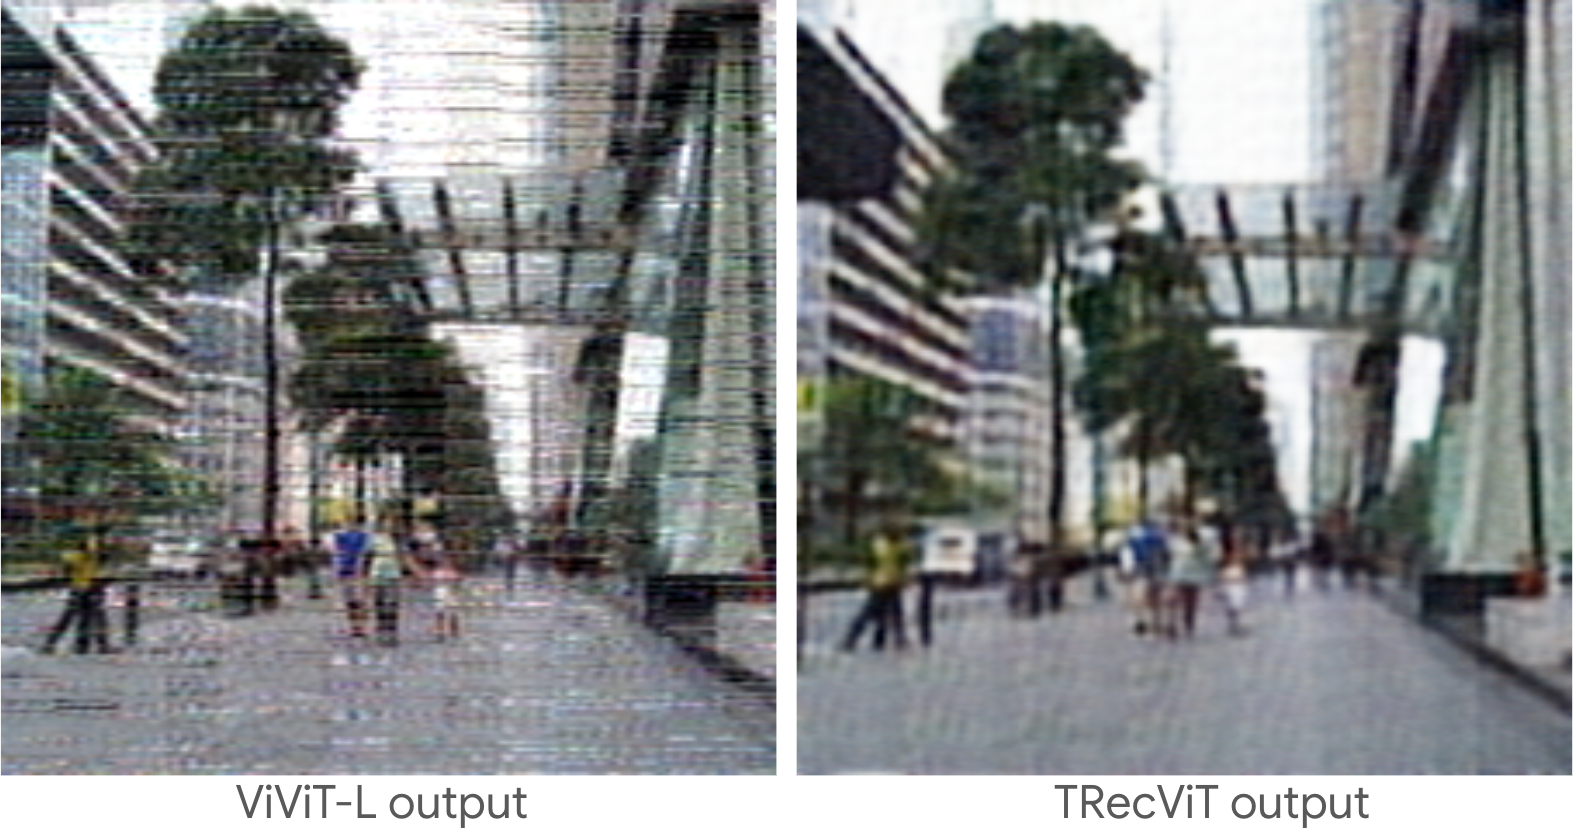
\includegraphics[width=\linewidth]{img/genlong.png}
  \caption{Generalisation to longer sequences. Both models are trained using Imagenet pre-trained weights, on video sequences of $T=64$ frames to reconstruct the $(T-48)^\text{th}$ frame; during evaluation, the models receive sequences of $T=96$ frames.}
  \label{fig:gentask}
\end{figure}

\section{Conclusion}
\label{sec:conclusion}
In this paper, we have investigated the common and unresolved issue that many established neural networks suffer from low floating-point operations per second (FLOPS). We have revisited a bottleneck operator, DWConv, and analyzed its main cause for a slowdown -- frequent memory access. To overcome the issue and achieve faster neural networks, we have proposed a simple yet fast and effective operator, PConv, that can be readily plugged into many existing networks. We have further introduced our general-purpose FasterNet, built upon our PConv, that achieves state-of-the-art speed and accuracy trade-off on various devices and vision tasks. We hope that our PConv and FasterNet would inspire more research on simple yet effective neural networks, going beyond academia to impact the industry and community directly.


{
    \small
    \bibliographystyle{ieeenat_fullname}
    \bibliography{main}
}

\newpage
\appendix

\section{Perception-Distortion Trade-Off}

\begin{figure}[b]
    \centering
    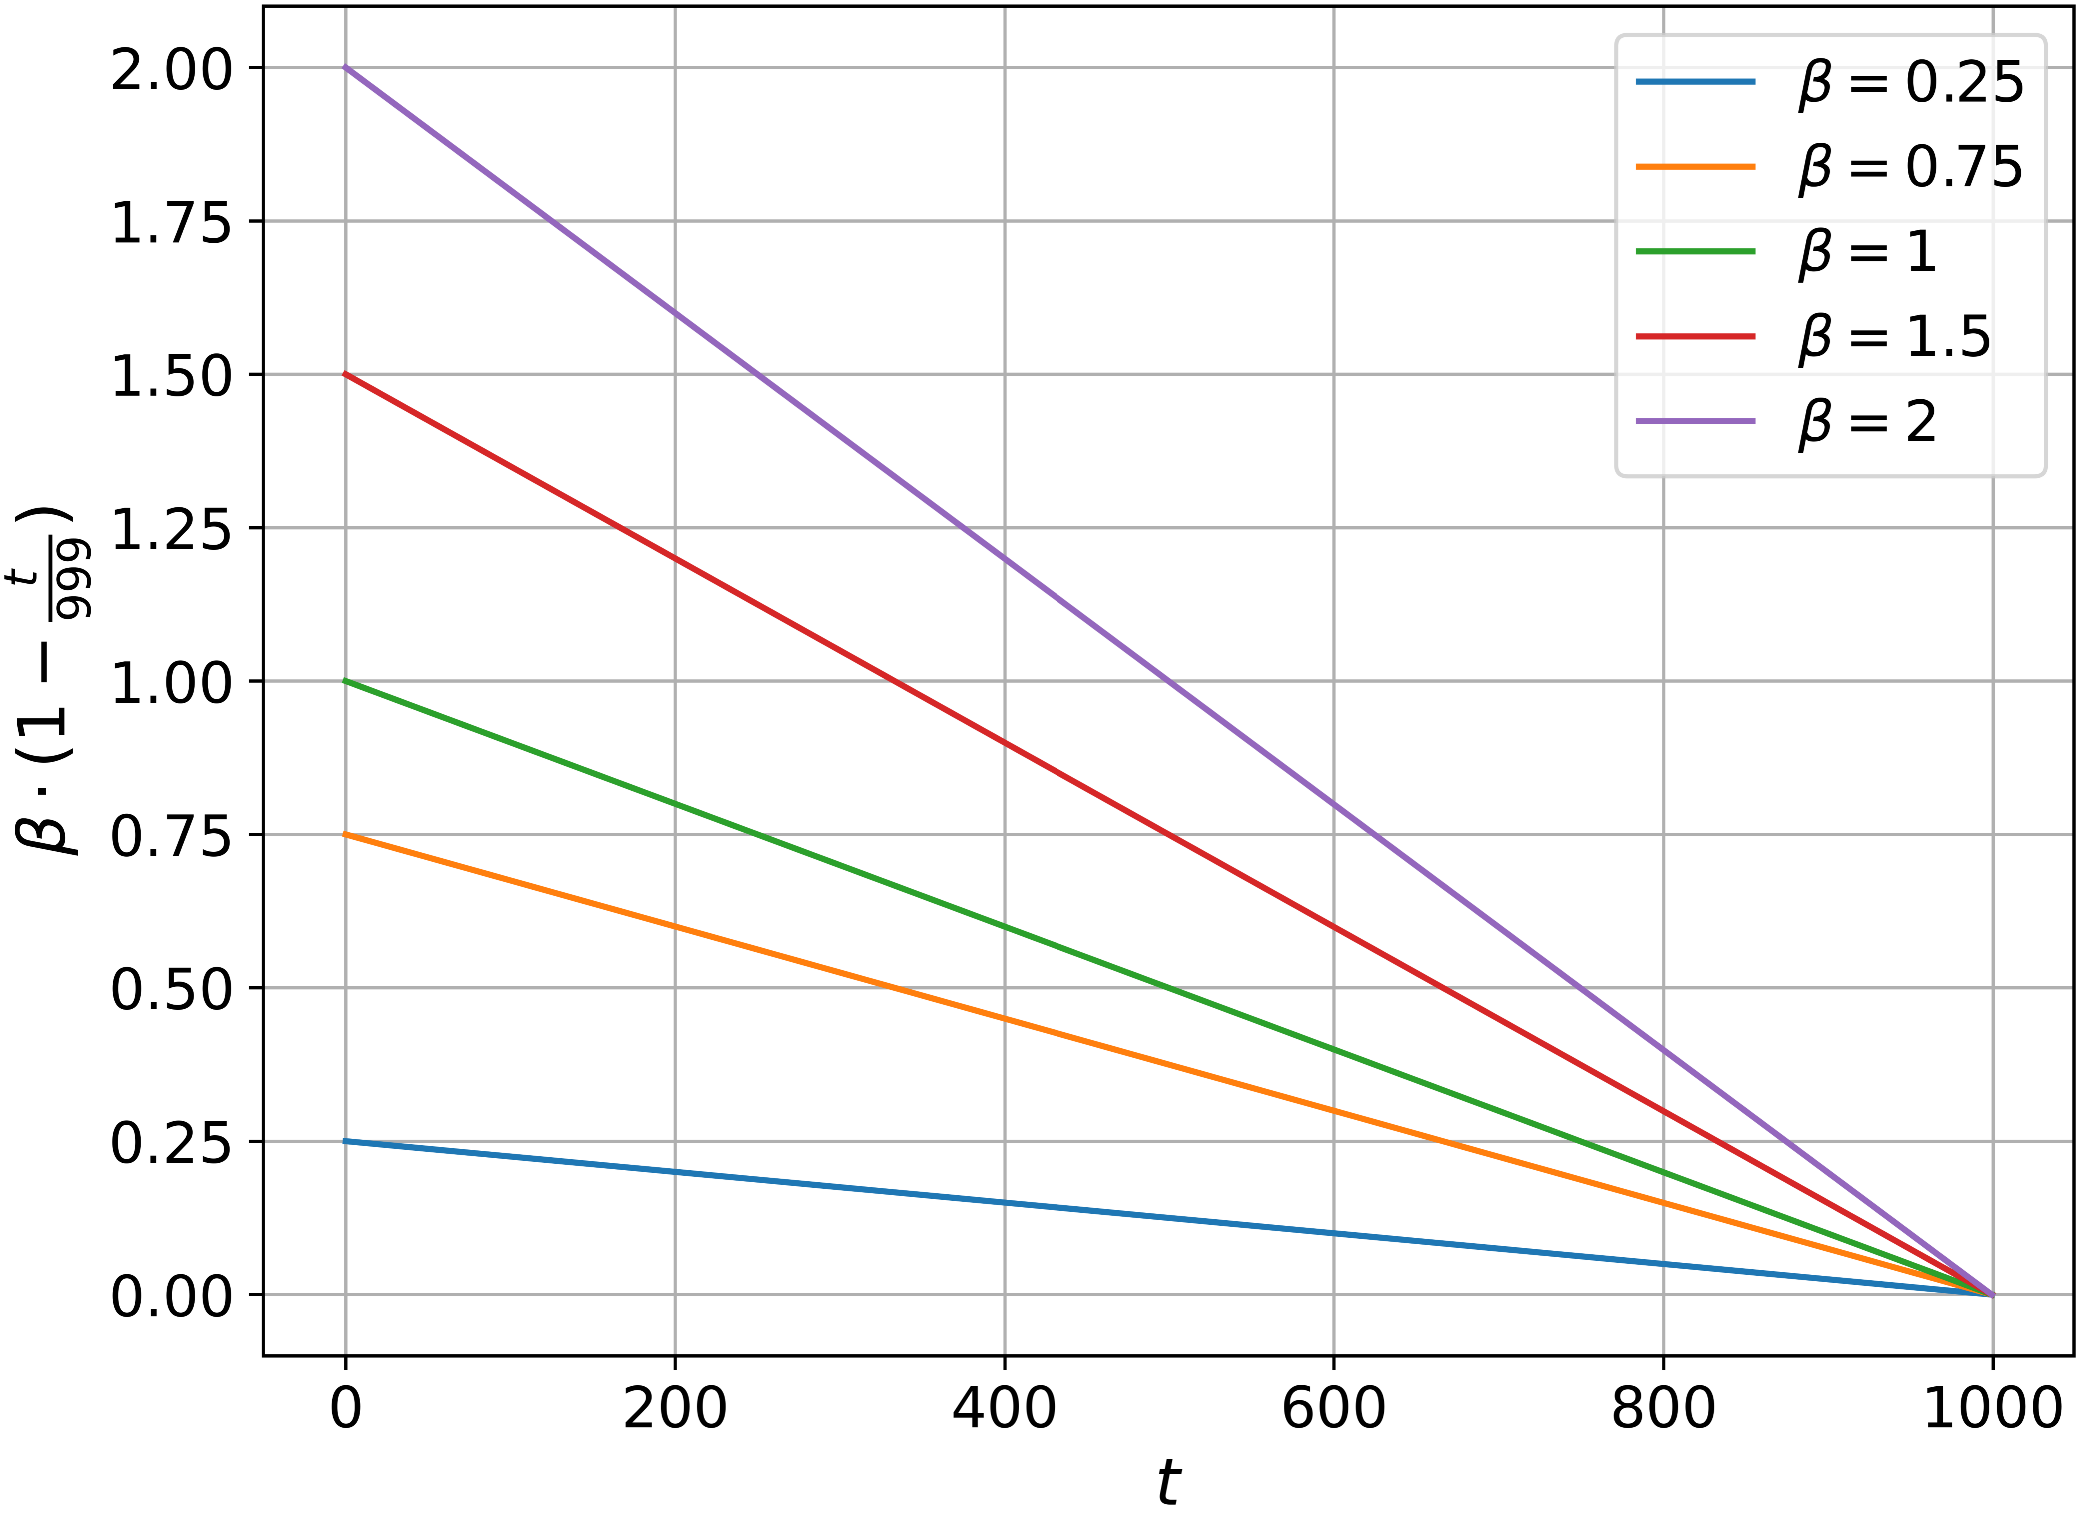
\includegraphics[width=1\linewidth]{figure_of_supp/bt_ablation.png}
    \caption{Ablation on $b(t)$. Higher hyper-parameter $\beta$ produces results with greater fidelity, while lower $\beta$ emphasizes more perceptual quality.}
    \label{fig:bt_ablation}
\end{figure}

The trade-off between perception and distortion \cite{blau2018perception} is a widely recognized challenge in the super-resolution domain. Thanks to our \textit{DF Loss}, our method can easily control the model to favor either fidelity or perceptual quality in the generated results. We can adjust the hyper-parameter $\beta$ in the $b(t)$ to achieve this goal. The total loss in our~\name~is:
\begin{equation}
    \mathcal{L}_{total} = \mathcal{L}_{v} + b(t)\mathcal{L}_{DF},
\end{equation}
The $b(t)$ can be written as follows:
\begin{equation}
    b(t) = \beta \cdot (1 - \frac{t}{t_{max}}),
\end{equation}
Where \( t \) is the timestep and \( \beta \) is the hyper-parameter that adjusts the weight between \( \mathcal{L}_v \) and \( \mathcal{L}_{DF} \), which we set to 1 by default. From equations (1) and (2), we can observe that a larger \( \beta \) increases the weight of the DF loss at each timestep, thereby further enhancing the fidelity of the results. In contrast, a smaller \( \beta \) reduces the influence of the DF loss at each timestep, allowing the v-prediction loss to have a greater impact and produce more perceptual results. The $b(t)$ - $t$ curves under different $\beta$ are shown in Figure \ref{fig:bt_ablation}. 

We conduct experiments under these settings to demonstrate the ability to achieve the perception-distortion trade-off. The quantitative results are shown in Table \ref{tab:beta_ablation}. From Table \ref{tab:beta_ablation}, we can observe that increasing $\beta$ improves the PSNR and $E_{warp}^*$, leading to better fidelity. Conversely, decreasing $\beta$ reduces the LPIPS score, indicating better perceptual quality.


\begin{table}[]
    \centering
    \caption{Qualitative comparison under different $\beta$ of $b(t)$.}
    \begin{tabular}{c|ccc}
    \hline
    $\beta$ & PSNR$\uparrow$ & LPIPS$\downarrow$ & $E_{warp}^*\downarrow$ \\ \hline
       0.25 & 23.55 & \textbf{0.1825} & 2.88  \\
       0.75 & 23.76 & 0.1842 & 2.74  \\
       1.0 & 23.91 & 0.1885 & 2.68  \\
       1.5 & 24.08 & 0.2272 & 2.53  \\
       2.0 & \textbf{24.41} & 0.3339 & \textbf{2.21} \\ \hline
    \end{tabular}
    \label{tab:beta_ablation}
\end{table}


\section{More Results}
\subsection{User Study}
To find the human-preferred results between our~\name~and other state-of-the-art methods, we conduct a user study that evaluate the results on both real-world and synthetic datasets. Specifically, we use the real-world dataset VideoLQ \cite{chan2022investigating} and the synthetic dataset REDS30 \cite{nah2019ntire}. We select two image-diffusion-model-based methods, Upscale-A-Video \cite{zhou2024upscale} and MGLD-VSR \cite{yang2023mgldvsr}; and one GAN-based method, RealViformer \cite{zhang2024realviformer} for comparison. 
We invite 12 evaluators to participate in the user study. For each evaluator, we randomly select 10 videos from each dataset and present four results: one from our~\name~and three from the compared methods. The evaluators were asked to choose which result had the best visual quality and temporal consistency.
The results of the user study are depicted in Figure \ref{fig:user_study}, indicating that our \name\ is preferred by most human evaluators for both visual quality and temporal consistency.

\begin{figure*}[]
    \centering
    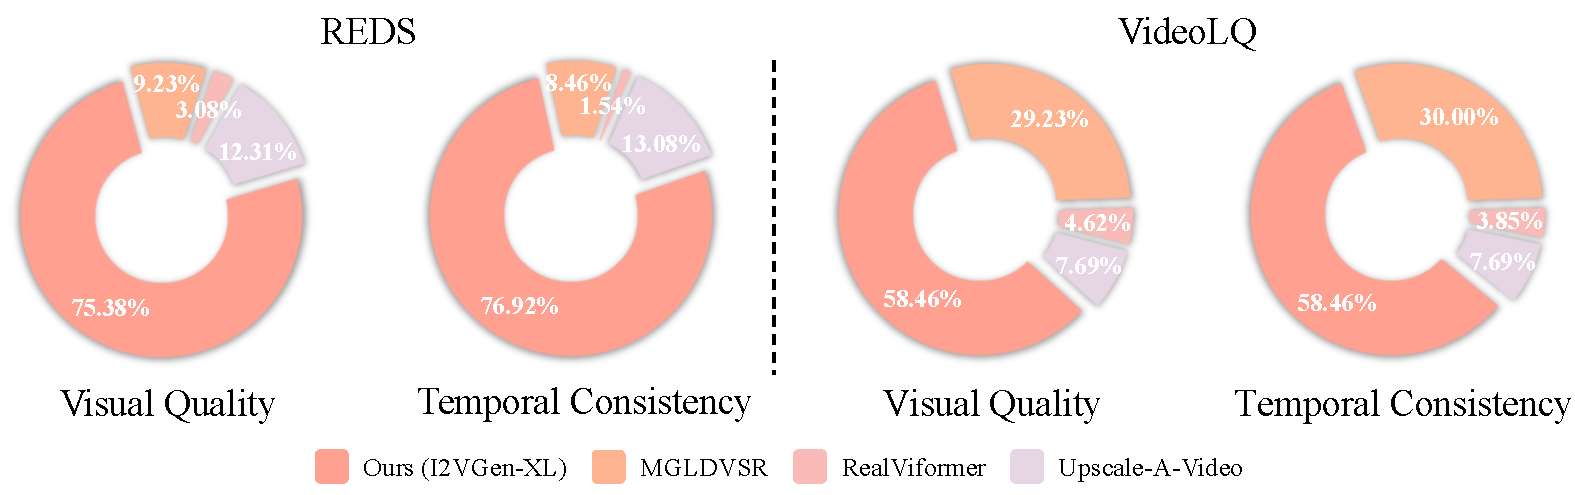
\includegraphics[width=\linewidth]{figure_of_supp/user_study.pdf}
    \caption{User study results. Our \name\ is preferred by human evaluators for both visual quality and temporal consistency.}
    \label{fig:user_study}
\end{figure*}


\begin{figure*}
    \centering
    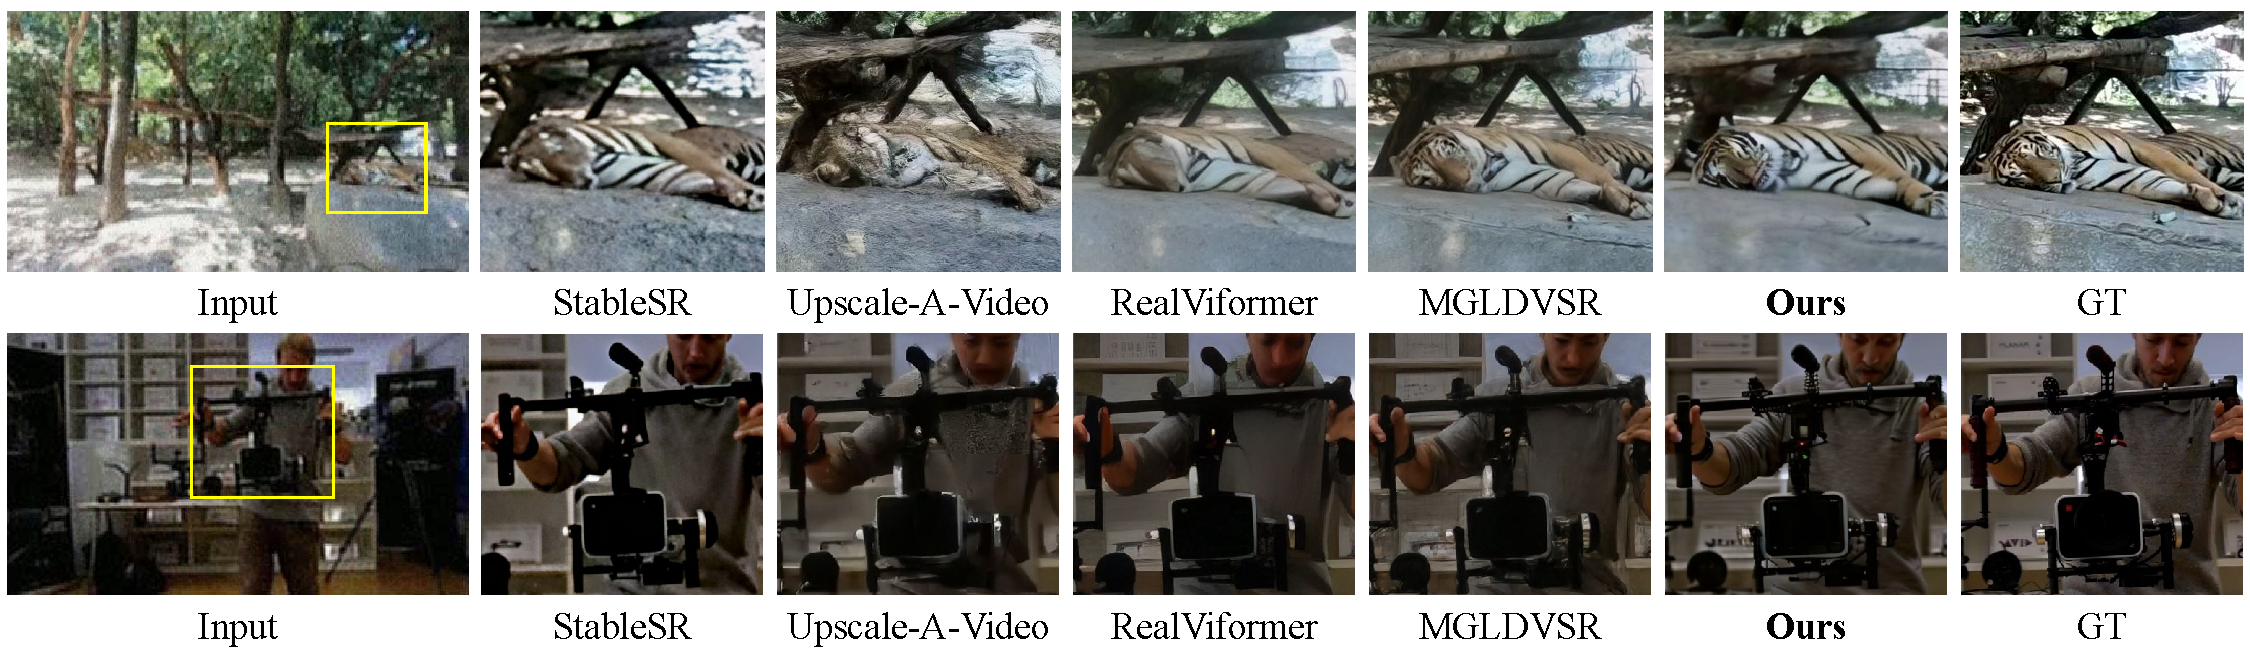
\includegraphics[width=1\linewidth]{figure_of_supp/synthetic.pdf}
    \caption{Qualitative comparisons on synthetic datasets. Our~\name~generates more detailed and realistic results. \textbf{(Zoom-in for best view)}}
    \label{fig:synthetic_comparison}
\end{figure*}

\begin{figure*}
    \centering
    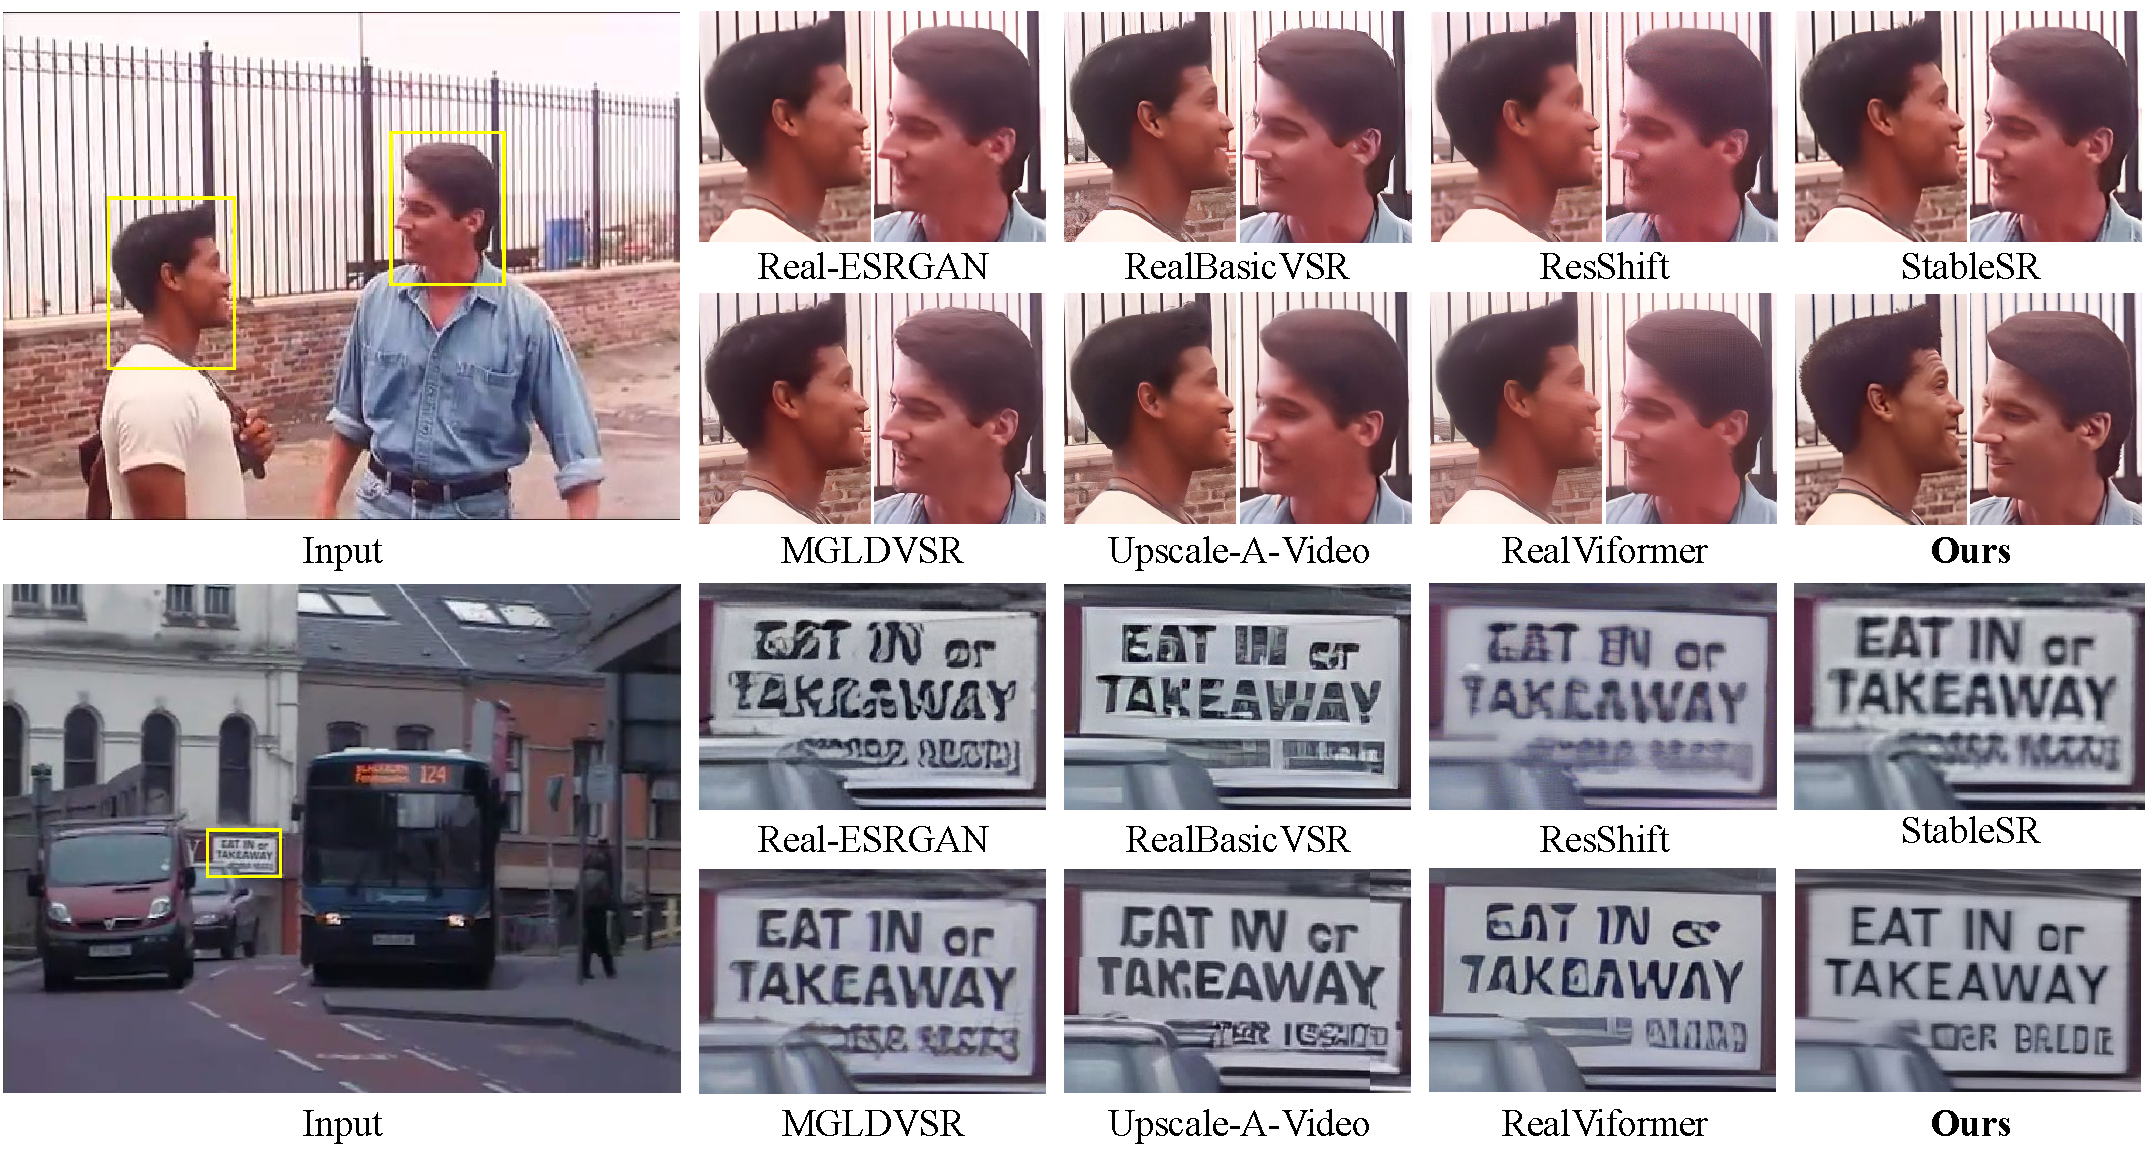
\includegraphics[width=1\linewidth]{figure_of_supp/real_world.pdf}
    \caption{Qualitative comparisons on real-world datasets. Our~\name~produces the clearest facial details and the most accurate text structure. \textbf{(Zoom-in for best view)}}
    \label{fig:realworld_comparison}
\end{figure*}

\begin{figure*}
    \centering
    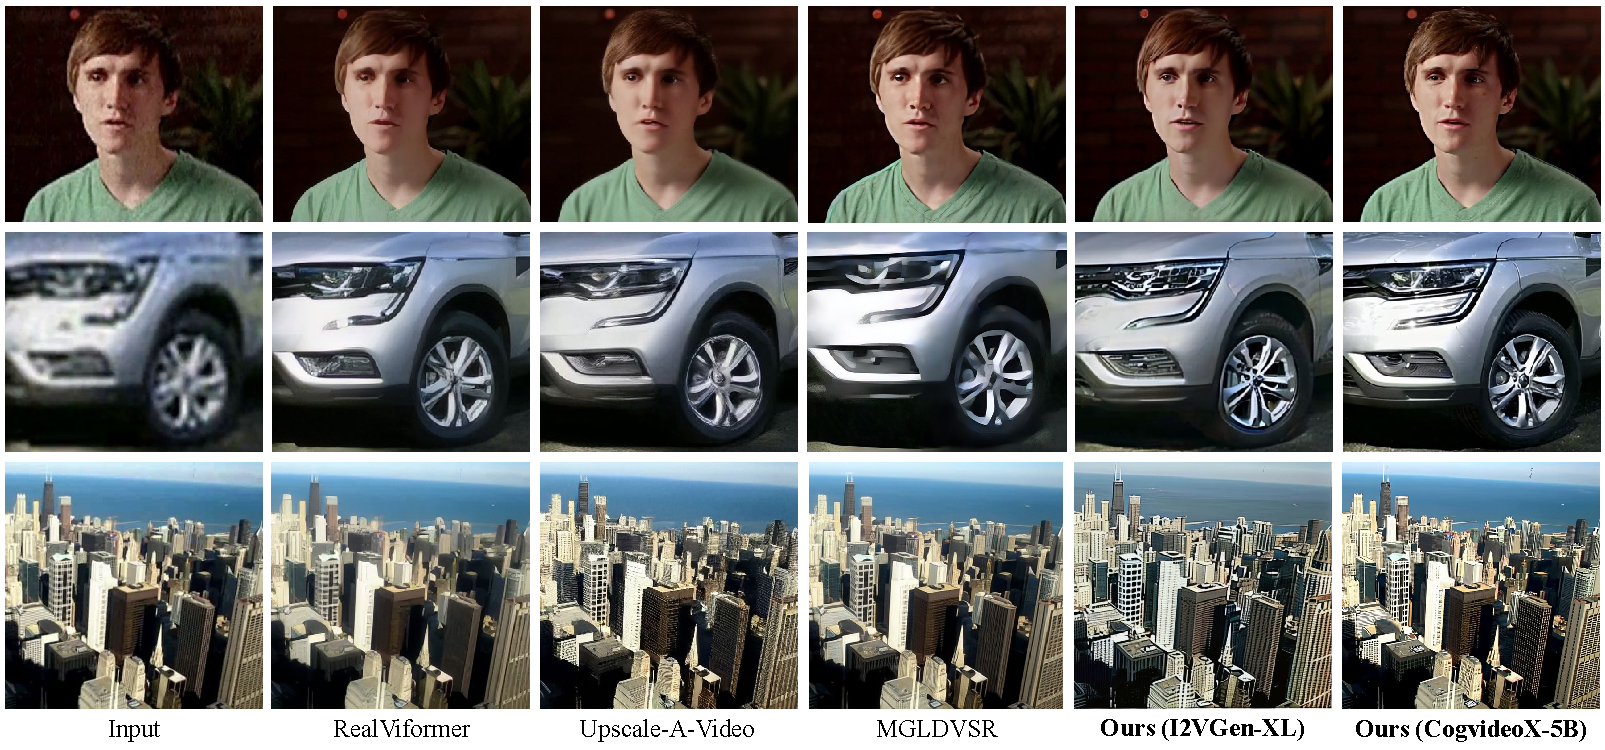
\includegraphics[width=1\linewidth]{figure_of_supp/scale_up.pdf}
    \caption{Qualitative comparisons on synthetic and real-world datasets with larger T2V models. Scaling up the T2V model enhances detail and realism in video super-resolution results. \textbf{(Zoom-in for best view)}}
    \label{fig:scale_up}
\end{figure*}

\subsection{Qualitative Comparisons}
We provide more visual comparisons on synthetic and real-world datasets in Figure \ref{fig:synthetic_comparison} and Figure \ref{fig:realworld_comparison} to further highlight our advantages in spatial quality. These results clearly demonstrate that our method preserves richer details and achieves greater realism.
To demonstrate the impact of scaling up with larger text-to-video (T2V) models, we present additional results in Figure \ref{fig:scale_up}. It is evident that scaling up the T2V model further improves the restoration effect, indicating that a large and robust T2V model can serve as a strong base model for video super-resolution.


\subsection{Video Demo}
We provide a demo video \href{https://youtu.be/hx0zrql-SrU}{\textcolor{red}{[STAR-demo.mp4]}} in the supplementary material, showcasing the temporal and spatial advantages of our proposed~\name~more intuitively. This video includes additional results and comparisons on synthetic, real-world, and AIGC videos.


\end{document}
